\documentclass[11pt]{article}

\usepackage[a4paper,margin=1in]{geometry}
\usepackage{amsmath,amssymb}
\usepackage{array}
\usepackage{booktabs}
\usepackage{graphicx}
\usepackage{hyperref}
\usepackage{placeins}

\graphicspath{{figures/}{report/figures/}}
\setlength{\emergencystretch}{2em}

\title{Primal--Dual Subgradient and Dual Averaging Experiments}
\author{}
\date{}

\begin{document}
\maketitle

\section{Introduction}
This report studies primal--dual subgradient methods for convex nonsmooth
optimization, with a focus on Nesterov's dual averaging framework
\cite{nesterov_primal_dual}.  The basic problem is
\[
    \min_{x\in Q} f(x),
\]
where \(Q\) is a closed convex set and \(f\) is convex but not necessarily
differentiable.  In such problems the oracle returns a subgradient
\(g\in\partial f(x)\).  Unlike gradients of smooth objectives, subgradients do
not generally vanish near an optimum.  This is the main reason classical
subgradient methods need decreasing primal step sizes.  At the same time, the
past subgradients define useful global affine lower models of the objective, so
discarding their information too quickly can be inefficient.

Dual averaging separates these two roles.  The method generates test points
\(x_0,x_1,\ldots\).  At each point \(x_i\), the oracle returns a subgradient
\(g_i\in\partial f(x_i)\), and the algorithm assigns this subgradient a
nonnegative averaging weight \(\lambda_i\).  The weighted average of past test
points is denoted by \(\hat x_k\).  The method accumulates subgradients in a
dual variable and obtains the next iterate \(x_{k+1}\) by regularizing this
accumulated linear model with a prox function.

Let \(d:Q\to\mathbb R\) be a strongly convex prox function with prox-center
\[
    x_0=\arg\min_{x\in Q} d(x),\qquad d(x_0)=0.
\]
The implementation starts from this prox-center, so the same \(x_0\) is also
the initial test point.
The parameter \(D>0\) defines the prox ball
\[
    F_D=\{x\in Q:\ d(x)\le D\}.
\]
In unrestricted SDA runs, \(D\) is used in the stopping certificate but the
iterate \(x_k\) may lie outside \(F_D\).  In restricted runs, the implementation
also projects iterates back to \(F_D\).

The associated prox mapping is
\[
    \pi_\beta(s)=
    \arg\min_{x\in Q}\{-\langle s,x\rangle+\beta d(x)\},
    \qquad \beta>0.
\]
For the Euclidean prox \(d(x)=\frac12\|x-x_0\|_2^2\), this reduces in the
unconstrained case to \(\pi_\beta(s)=x_0+s/\beta\).

The generic dual averaging update is
\[
    s_{k+1}=s_k+\lambda_k g_k,
    \qquad
    x_{k+1}=\pi_{\beta_{k+1}}(-s_{k+1}),
\]
where \(s_k\) is the accumulated dual vector and \(\beta_{k+1}>0\) controls the
strength of the prox regularization.

The primal--dual feature of the method is the computable certificate
\[
    \delta_k(D)=
    \max_{x\in F_D}\sum_{i=0}^k \lambda_i
    \langle g_i,x_i-x\rangle ,
    \qquad
    S_k=\sum_{i=0}^k\lambda_i .
\]
If the selected radius satisfies the required condition
\[
    D\ge d(x^\star),
\]
then \(x^\star\in F_D\) and the normalized primal--dual certificate gap
\(\delta_k(D)/S_k\) bounds the objective error of the averaged iterate
\(\hat x_k\).  This
radius condition is essential: when \(x^\star\notin F_D\), the certificate is no
longer a valid certificate for the original problem and can even become
negative.  The experiments therefore distinguish the primal--dual certificate
gap from the benchmark objective gap \(f(\hat x_k)-f^\star\) and from the lasso
train-objective gap \(F(\hat x_k)-F(x_{\mathrm{saga}})\).

The implemented methods are simple dual averaging (SDA), weighted SDA,
stochastic simple averages (SSA), and a projected subgradient baseline.  The
deterministic benchmark experiments use nonsmooth convex objectives with known
optima, so their objective gap is \(f(\hat x_k)-f^\star\).  The lasso logistic
experiments use empirical train objectives and compare against a matched
\texttt{sklearn} SAGA reference; their reported train-objective gap is
\(F(\hat x_k)-F(x_{\mathrm{saga}})\).  This distinction is used throughout the
report.

\section{Implemented Methods}
\subsection{Shared Dual Averaging State}

This section describes the implementation using the same notation as the code.
The common inputs are an initial point \(x_0\), a prox-radius parameter \(D\), a
maximum iteration count, a subgradient oracle \(G\), a step multiplier
\(\gamma_{\mathrm{mult}}\) for the SDA variants, and, for deterministic SDA, a
stopping tolerance \(\varepsilon\).  The boolean option
\texttt{restrict\_to\_fd} controls whether each new iterate is projected back to
\(F_D\).  If this option is false, \(D\) is still used in the primal--dual
certificate gap, but it does not constrain the iterates.

\begin{center}
\small
\begin{tabular}{ll}
\toprule
Symbol & Meaning \\
\midrule
\(x_k\) & primal test point at iteration \(k\) \\
\(g_k\) & subgradient returned at \(x_k\), usually \(g_k\in\partial f(x_k)\) \\
\(\lambda_k\) & dual averaging weight assigned to \(g_k\) \\
\(s_k\) & accumulated dual vector \\
\(S_k\) & accumulated averaging weight \\
\(\hat x_k\) & weighted average of past primal test points \\
\(D\) & prox-radius parameter defining \(F_D=\{x:d(x)\le D\}\) \\
\(\delta_k(D)/S_{k+1}\) & normalized primal--dual certificate gap used for deterministic SDA stopping \\
\(\gamma\) & prox scale used in \(B_{k+1}=\gamma\hat\beta_{k+1}\) \\
\(\gamma_{\mathrm{mult}}\) & dimensionless multiplier applied to the baseline \(\gamma^\star\) \\
\bottomrule
\end{tabular}
\end{center}

The implementation stores the state after processing iteration \(k\) at index
\(k+1\).  Thus the denominator \(S_{k+1}\) below contains the weights
\(\lambda_0,\ldots,\lambda_k\), which is the same accumulated quantity denoted
by \(S_k=\sum_{i=0}^k\lambda_i\) in the introductory certificate formula.

All dual averaging variants maintain a sequence of primal test points
\(\{x_k\}\), subgradients \(g_k\in\partial f(x_k)\), nonnegative weights
\(\lambda_k\), the accumulated dual vector
\[
    s_{k+1}=s_k+\lambda_k g_k,\qquad s_0=0,
\]
and the accumulated weight
\[
    S_{k+1}=S_k+\lambda_k,\qquad S_0=0.
\]
The averaged primal point is updated as
\[
    \hat x_{k+1}
    =
    \frac{S_k\hat x_k+\lambda_k x_k}{S_{k+1}}.
\]
The implementation also stores
\[
    \delta_k(D)
    =
    \sum_{i=0}^k\lambda_i\langle g_i,x_i-x_0\rangle
    +\xi_D(-s_{k+1}),
\]
where
\[
    \xi_D(s)=\max_{x\in F_D}\langle s,x-x_0\rangle .
\]
The quantity \(\delta_k(D)/S_{k+1}\) is the primal--dual certificate gap used
for deterministic SDA stopping.  It is not the same metric as the benchmark
objective gap or the lasso train-objective gap to SAGA.

The code implements three prox geometries.  For the Euclidean prox,
\[
    d(x)=\frac12\|x-x_0\|_2^2,
    \qquad
    \xi_D(s)=\sqrt{2D}\|s\|_2.
\]
For the weighted Euclidean prox with positive diagonal weights \(h_i\),
\[
    d(x)=\frac12\sum_i h_i(x_i-x_{0,i})^2,
    \qquad
    \xi_D(s)=\sqrt{2D\sum_i s_i^2/h_i}.
\]
For the entropy prox on the probability simplex,
\[
    d(x)=\log n+\sum_{i=1}^n x_i\log x_i,
    \qquad
    x_0=(1/n,\ldots,1/n).
\]
All implemented prox functions are treated as having strong convexity parameter
\(\sigma=1\).  Nesterov's SDA bound contains the expression
\[
    \gamma D+\frac{L^2}{2\sigma\gamma}.
\]
Balancing these two terms gives the baseline scale
\[
    \gamma^\star=\frac{L}{\sqrt{2\sigma D}}=\frac{L}{\sqrt{2D}},
\]
where \(L\) is the Lipschitz estimate supplied by the objective wrapper.  The
implementation then uses
\[
    \gamma=\gamma^\star\gamma_{\mathrm{mult}}.
\]
The multiplier \(\gamma_{\mathrm{mult}}\) is dimensionless and is used for
tuning around the theoretical baseline.  Larger \(\gamma\) increases the prox
regularization and makes the accumulated subgradient model move the iterate
less aggressively; smaller \(\gamma\) weakens this regularization and produces
larger primal moves.

\subsection{Simple Dual Averaging}

Simple Dual Averaging uses unit aggregation weights,
\[
    \lambda_k=1.
\]
The scale sequence follows Nesterov's recurrence
\[
    \hat\beta_0=\hat\beta_1=1,
    \qquad
    \hat\beta_{k+1}=\hat\beta_k+\frac{1}{\hat\beta_k},
\]
and the implementation sets
\[
    B_{k+1}=\gamma\hat\beta_{k+1}.
\]
Here \(B_{k+1}\) is the implementation name for the prox parameter
\(\beta_{k+1}\) in the mapping \(\pi_{\beta_{k+1}}\).
The primal update is
\[
    x_{k+1}=\pi_{B_{k+1}}(-s_{k+1}).
\]
For unconstrained Euclidean runs this is
\[
    x_{k+1}=x_0-\frac{s_{k+1}}{B_{k+1}}.
\]

\paragraph{Pseudocode.}
\begin{enumerate}
    \item Choose \(x_0\), \(D\), \(\varepsilon\), \(\gamma_{\mathrm{mult}}\),
    and a maximum iteration count.  Set \(s_0=0\), \(S_0=0\), and
    \(\hat x_0=x_0\).  Set \(\hat\beta_0=\hat\beta_1=1\).
    \item Set \(\gamma=\gamma^\star\gamma_{\mathrm{mult}}\), where
    \(\gamma^\star=L/\sqrt{2D}\).
    \item For \(k=0,1,\ldots\):
    \begin{enumerate}
        \item compute \(g_k\in\partial f(x_k)\);
        \item set \(\lambda_k=1\), \(s_{k+1}=s_k+g_k\), and
        \(S_{k+1}=S_k+1\);
        \item use \(\hat\beta_1=1\) for \(k=0\), and for later iterations
        update \(\hat\beta_{k+1}=\hat\beta_k+1/\hat\beta_k\); set
        \(B_{k+1}=\gamma\hat\beta_{k+1}\), and compute
        \(x_{k+1}=\pi_{B_{k+1}}(-s_{k+1})\);
        \item optionally project \(x_{k+1}\) to \(F_D\) in restricted runs;
        \item update \(\hat x_{k+1}\) and compute
        \(\delta_k(D)/S_{k+1}\);
        \item stop if the deterministic primal--dual certificate gap is at
        most \(\varepsilon\).
    \end{enumerate}
\end{enumerate}

\subsection{Weighted Dual Averaging}

Weighted SDA uses the same primal update and the same \(\hat\beta_k\) sequence
as simple SDA, but changes the aggregation weights to
\[
    \lambda_k=
    \begin{cases}
        1/\|g_k\|_*, & \|g_k\|_*>0,\\
        0, & \|g_k\|_*=0.
    \end{cases}
\]
This gives each nonzero subgradient a unit dual-norm contribution in the dual
aggregate, since \(\|\lambda_k g_k\|_*=1\).  The zero-subgradient convention
prevents division by zero.
Nesterov's weighted dual averages method is parameterized by \(\rho\), whereas
the implementation exposes the same \(\gamma\) interface used by SDA.  Since
the implemented prox functions use \(\sigma=1\), the code treats
\[
    \rho=\frac{1}{\gamma},
    \qquad
    \gamma=\gamma^\star\gamma_{\mathrm{mult}}.
\]
Thus \(\gamma_{\mathrm{mult}}\) still controls the practical scale of the
prox regularization, but the weighted method should be interpreted through the
paper's inverse \(\rho\) convention.

\paragraph{Pseudocode.}
\begin{enumerate}
    \item Initialize \(x_0\), \(s_0=0\), \(S_0=0\), \(\hat x_0=x_0\), and
    \(\gamma=\gamma^\star\gamma_{\mathrm{mult}}\).  Set
    \(\hat\beta_0=\hat\beta_1=1\).
    \item For \(k=0,1,\ldots\):
    \begin{enumerate}
        \item compute \(g_k\in\partial f(x_k)\);
        \item compute \(\lambda_k=1/\|g_k\|_*\), using \(\lambda_k=0\) if
        \(g_k=0\);
        \item update \(s_{k+1}=s_k+\lambda_k g_k\) and
        \(S_{k+1}=S_k+\lambda_k\);
        \item use the same \(\hat\beta_k\) recursion as simple SDA and compute
        \(x_{k+1}=\pi_{\gamma\hat\beta_{k+1}}(-s_{k+1})\);
        \item optionally project \(x_{k+1}\) to \(F_D\) in restricted runs;
        \item update \(\hat x_{k+1}\) using the weighted average and compute
        the primal--dual certificate gap;
        \item stop if the deterministic primal--dual certificate gap is at
        most \(\varepsilon\).
    \end{enumerate}
\end{enumerate}

\subsection{Stochastic Simple Averages}

SSA is the stochastic version of simple dual averaging.  Instead of evaluating
a full deterministic subgradient, the method draws an independent random
sample \(\xi_k\) and uses
\[
    \tilde g_k=G(x_k,\xi_k).
\]
For the finite-sum lasso logistic objective, \(\xi_k\) is a training-row index
sampled with replacement.  The experiments use batch size one, so the sampled
logistic gradient for the feature coordinates is
\[
    a_{\xi_k}\left(\sigma(a_{\xi_k}^{\mathsf T}w+b)-y_{\xi_k}\right),
\]
where \(a_{\xi_k}\) is the sampled feature vector.  The intercept coordinate is
\[
    \sigma(a_{\xi_k}^{\mathsf T}w+b)-y_{\xi_k}.
\]
The same deterministic lasso subgradient term is then added using the
\(\lambda/n\) scaling of the full objective, where \(\lambda\) is the lasso
regularization parameter and is unrelated to the dual averaging weights
\(\lambda_k\).  The sampled logistic gradient is an unbiased estimator of the
empirical logistic gradient component, while the lasso term is deterministic at
the current iterate.  The SSA implementation uses the SDA recursion with
\(\lambda_k=1\), but disables stopping on the sampled primal--dual certificate
gap because that per-run quantity is noisy and is not the deterministic
certificate used by full-gradient SDA.  The sampled certificate is still
tracked internally for diagnostics.

\paragraph{Pseudocode.}
\begin{enumerate}
    \item Initialize \(x_0\), \(s_0=0\), \(S_0=0\), \(\hat x_0=x_0\), random
    seed, and \(\gamma=\gamma^\star\gamma_{\mathrm{mult}}\).  Set
    \(\hat\beta_0=\hat\beta_1=1\).
    \item For \(k=0,1,\ldots,\texttt{max\_iter}-1\):
    \begin{enumerate}
        \item sample a training index or mini-batch \(\xi_k\);
        \item compute the stochastic subgradient \(\tilde g_k=G(x_k,\xi_k)\);
        \item set \(s_{k+1}=s_k+\tilde g_k\), \(S_{k+1}=S_k+1\);
        \item use the same \(\hat\beta_k\) recursion as simple SDA and compute
        \(x_{k+1}=\pi_{\gamma\hat\beta_{k+1}}(-s_{k+1})\);
        \item update the simple average \(\hat x_{k+1}\).
    \end{enumerate}
\end{enumerate}

\subsection{Projected Subgradient Baseline}

The baseline method is Euclidean projected subgradient descent.  It uses
\[
    \alpha_k=\frac{\alpha}{\sqrt{k+1}},
    \qquad
    x_{k+1}=x_k-\alpha_k g_k.
\]
When a restricted run is requested, \(x_{k+1}\) is projected to the Euclidean
prox ball \(F_D=\{x:\frac12\|x-x_0\|_2^2\le D\}\).  The method tracks the same
averaged iterate \(\hat x_k\) for metric reporting, but it does not compute a
dual averaging primal--dual certificate gap.

\paragraph{Pseudocode.}
\begin{enumerate}
    \item Choose \(x_0\), \(\alpha\), \(D\), and \(\texttt{max\_iter}\).
    \item For \(k=0,1,\ldots,\texttt{max\_iter}-1\):
    \begin{enumerate}
        \item compute \(g_k\in\partial f(x_k)\);
        \item set \(\alpha_k=\alpha/\sqrt{k+1}\);
        \item update \(x_{k+1}=x_k-\alpha_k g_k\);
        \item optionally project \(x_{k+1}\) to \(F_D\);
        \item update the arithmetic average \(\hat x_{k+1}\).
    \end{enumerate}
\end{enumerate}

\subsection{Objective Definitions}

The nonsmooth benchmark registry contains convex objectives with known
reference optima.  The Euclidean benchmark grid uses the nine objectives in
Table~\ref{tab:benchmark-objectives}; the simplex entropy experiment uses the
three objectives in Table~\ref{tab:simplex-objectives}.  The deterministic
subgradient convention at nondifferentiable ties is fixed by the implementation:
absolute-value terms use sign zero at exactly zero, and max-affine objectives
select one active affine piece.

\begin{table}[htbp]
\centering
\scriptsize
\begin{tabular}{@{}p{0.23\textwidth}p{0.34\textwidth}p{0.36\textwidth}@{}}
\toprule
Objective id & Definition & Parameters used \\
\midrule
\path{abs_a2}
& \(f(x)=|x-a|\)
& \(a=2\). \\
\path{weighted_l1_shift_1d}
& \(f(x)=\sum_{j=1}^3 w_j|x-a_j|\)
& \(w=(1.25,0.75,0.5)\), \(a=(2,-1.5,3.5)\). \\
\path{max_affine_1d}
& \(f(x)=\max_j\{m_jx+b_j\}\)
& \(m=(1.2,-0.8,0.35)\), \(b=(-2,2.6,0.9)\). \\
\path{weighted_l1_shift_2d}
& \(f(x)=\sum_{i=1}^2 w_i|x_i-a_i|\)
& \(w=(1,1.5)\), \(a=(2,-1)\). \\
\path{linf_shift_2d}
& \(f(x)=\max_i |x_i-a_i|\)
& \(a=(1.5,-2.5)\). \\
\path{weighted_l1_shift_4d}
& \(f(x)=\sum_{i=1}^4 w_i|x_i-a_i|\)
& \(w=(1,0.5,1.25,0.75)\), \(a=(2.5,-1.5,1,3)\). \\
\path{max_affine_4d}
& \(f(x)=\max_j\{a_j^{\mathsf T}x+b_j\}\)
& Rows \(a_j=e_1,e_2,e_3,e_4,-\mathbf 1\), \(b=(-2,1.5,-0.75,-2.5,3.75)\). \\
\path{ill_conditioned_l1_shift_8d}
& \(f(x)=\sum_{i=1}^8 w_i|x_i-a_i|\)
& \(w=(0.1,0.2,0.5,1,2,5,10,25)\), \(a=(2,-1.5,1,3,-2,0.5,1.5,-0.75)\). \\
\path{ill_conditioned_max_affine_8d}
& \(f(x)=\max_i c_i|x_i-a_i|\)
& \(c=(0.1,0.2,0.5,1,2,5,10,25)\), \(a=(2,-1.5,1,3,-2,0.5,1.5,-0.75)\). \\
\bottomrule
\end{tabular}
\caption{Nonsmooth Euclidean benchmark objectives.}
\label{tab:benchmark-objectives}
\end{table}

The simplex objectives are defined on
\[
    \Delta_n=\{x\in\mathbb R^n:\ x_i\ge0,\ \sum_i x_i=1\}.
\]
For max-affine simplex objectives, the objective is
\[
    f(x)=\max_j\{a_j^{\mathsf T}x+b_j\}.
\]

\begin{table}[htbp]
\centering
\scriptsize
\begin{tabular}{@{}p{0.23\textwidth}p{0.25\textwidth}p{0.44\textwidth}@{}}
\toprule
Objective id & Definition & Parameters used \\
\midrule
\path{simplex_linear_8d}
& \(f(x)=c^{\mathsf T}x\), \(x\in\Delta_8\)
& \(c=(0.8,-0.4,1.2,0.1,-0.9,0.3,0.6,-0.2)\). \\
\path{simplex_max_affine_8d}
& \(f(x)=\max_{1\le j\le6}\{a_j^{\mathsf T}x+b_j\}\), \(x\in\Delta_8\)
& \(b=(0,0.1,-0.05,0.2,-0.1,0.05)\).  The six rows \(a_j\) are
\((1,-0.5,0.2,0,-0.3,0.4,0.1,-0.2)\),
\((-0.4,0.8,-0.1,0.3,0.2,-0.5,0.6,0)\),
\((0.2,0.1,0.9,-0.4,0.5,0,-0.3,0.4)\),
\((0,-0.2,0.4,1,-0.5,0.3,0.2,-0.1)\),
\((-0.3,0.4,0,-0.2,0.9,-0.1,0.5,0.2)\),
\((0.5,0,-0.4,0.2,0.1,0.8,-0.2,0.3)\). \\
\path{simplex_sparse_max_affine_16d}
& \(f(x)=\max_{1\le j\le16}\{a_j^{\mathsf T}x+b_j\}\), \(x\in\Delta_{16}\)
& \(b_j=0.02(j-1)\).  For \(j=1,\ldots,8\), row \(a_j\) has \(1\) in coordinate \(j\), \(-0.2\) in coordinate \(j+1\), and zeros elsewhere.  For \(j=9,\ldots,16\), row \(a_j\) has \(-0.5\) in coordinate \(j-8\), \(0.7\) in coordinate \(j-4\), and zeros elsewhere. \\
\bottomrule
\end{tabular}
\caption{Simplex benchmark objectives used with entropy prox.}
\label{tab:simplex-objectives}
\end{table}

For logistic regression, let \(a_i\in\mathbb R^p\) be the feature vector and
\(y_i\in\{0,1\}\) the binary label.  The lasso logistic objective used in the
experiments is
\[
    F(w,b)=
    \frac1n\sum_{i=1}^n
    \left[
        \log(1+\exp(a_i^{\mathsf T}w+b))
        -y_i(a_i^{\mathsf T}w+b)
    \right]
    +\frac{\lambda}{n}\|w\|_1 .
\]
The intercept \(b\) is appended as the final coordinate of the optimization
vector and is not penalized.  Here \(\lambda\) denotes the lasso
regularization parameter, not a dual averaging weight.  The implementation
first loads numeric CSV features with binary labels, creates a stratified
train/test split, standardizes features using train-set statistics only, and
then appends a bias column.

\subsection{Logistic Regression Datasets}

The synthetic datasets were generated by \texttt{data/generate\_logistic\_data.py}.
The generator takes the number of samples, feature dimension, coefficient
vector \(\beta\), intercept \(b\), random seed, label-flip probability, and
output path.  It samples features
\[
    a_i\sim N(0,I),
\]
forms logits \(a_i^{\mathsf T}\beta+b\), samples
\(y_i\sim\mathrm{Bernoulli}(\sigma(a_i^{\mathsf T}\beta+b))\), and then flips
each label independently with probability \(p_{\mathrm{flip}}\).  The recorded
synthetic parameters are shown in Table~\ref{tab:synthetic-dataset-params}.
The two larger synthetic datasets are included to stress the weighted SDA
versus SSA comparison on larger finite-sum lasso objectives.

The public datasets are downloaded and normalized by the script
\path{data/download_binary_datasets.py}.  They all use the same normalized
schema: numeric feature columns and a binary label column.  The Iris dataset is
converted to Setosa versus non-Setosa classification.  The Wisconsin Diagnostic
Breast Cancer dataset classifies malignant versus benign tumors.  The Banknote
Authentication dataset classifies genuine versus forged banknotes from image
features.  The Spambase dataset classifies email as spam or non-spam.

\begin{table}[htbp]
\centering
\small
\resizebox{\textwidth}{!}{%
\begin{tabular}{llrrl}
\toprule
Dataset & Type & Samples & Features & Description \\
\midrule
\texttt{iris.csv} & UCI public & 150 & 4 & Setosa versus non-Setosa Iris classification \\
\texttt{breast\_cancer\_wdbc.csv} & UCI public & 569 & 30 & malignant versus benign tumor classification \\
\texttt{banknote\_authentication.csv} & UCI public & 1372 & 4 & genuine versus forged banknote classification \\
\texttt{spambase.csv} & UCI public & 4601 & 57 & spam versus non-spam email classification \\
\texttt{synthetic\_logistic\_small\_5d.csv} & synthetic & 240 & 5 & small balanced sanity-check dataset \\
\texttt{synthetic\_logistic\_sparse\_20d.csv} & synthetic & 1000 & 20 & sparse informative coordinates, no label flips \\
\texttt{synthetic\_logistic\_noisy\_20d.csv} & synthetic & 1000 & 20 & same sparse structure with 10\% label flips \\
\texttt{synthetic\_logistic\_imbalanced\_10d.csv} & synthetic & 800 & 10 & shifted intercept and 3\% label flips \\
\texttt{synthetic\_logistic\_big\_sparse\_50d.csv} & synthetic & 12000 & 50 & larger sparse synthetic lasso comparison dataset \\
\texttt{synthetic\_logistic\_big\_noisy\_80d.csv} & synthetic & 20000 & 80 & larger noisy synthetic lasso comparison dataset \\
\bottomrule
\end{tabular}
}
\caption{Logistic regression datasets used by the lasso experiments.}
\label{tab:logistic-datasets}
\end{table}

\begin{table}[htbp]
\centering
\scriptsize
\resizebox{\textwidth}{!}{%
\begin{tabular}{lrrrrrl}
\toprule
Dataset & Samples & Dim. & Intercept & Seed & Flip prob. & Coefficient vector \(\beta\) \\
\midrule
\path{synthetic_logistic_small_5d.csv}
& 240 & 5 & 0 & 10 & 0
& \((2,-1.5,1,-0.5,0.25)\) \\
\path{synthetic_logistic_sparse_20d.csv}
& 1000 & 20 & 0 & 20 & 0
& \((2.5,-2,1.5,-1,0.75,0.5,0,\ldots,0)\) \\
\path{synthetic_logistic_noisy_20d.csv}
& 1000 & 20 & 0 & 21 & 0.10
& \((2.5,-2,1.5,-1,0.75,0.5,0,\ldots,0)\) \\
\path{synthetic_logistic_imbalanced_10d.csv}
& 800 & 10 & -1.2 & 30 & 0.03
& \((1.5,-1.25,1,-0.75,0.5,0.25,0,\ldots,0)\) \\
\path{synthetic_logistic_big_sparse_50d.csv}
& 12000 & 50 & 0 & 50 & 0
& \((3,-2.5,2,-1.5,1.2,-1,0.8,-0.6,0.4,-0.3,0,\ldots,0)\) \\
\path{synthetic_logistic_big_noisy_80d.csv}
& 20000 & 80 & -0.4 & 80 & 0.15
& \((2.5,-2.2,1.8,-1.5,1.2,-1,0.8,-0.6,0.5,-0.4,0.3,-0.2,0,\ldots,0)\) \\
\bottomrule
\end{tabular}
}
\caption{Synthetic logistic dataset generation parameters.}
\label{tab:synthetic-dataset-params}
\end{table}

\section{Experiments}
\label{sec:experiments}

This section reports the experiments conducted for the implemented subgradient and
dual-averaging solvers.  The benchmark experiments use convex nonsmooth test
objectives with known reference optima, so their plotted objective gap is
\[
    f(\hat x_k)-f^\star ,
\]
where \(\hat x_k\) is the averaged primal iterate.  The lasso logistic
experiments do not have a closed-form optimum.  For those runs, the reference
value is the train objective achieved by a matched \texttt{sklearn} SAGA run,
and the plotted train-objective gap is
\[
    F(\hat x_k)-F(x_{\mathrm{saga}}).
\]
Small negative lasso train-objective gaps should therefore be read as numerical
ties with the SAGA reference, not as proof that the global optimum has been
beaten.  SDA also computes a separate primal--dual certificate gap
\(\delta_k(D)/S_k\), which is used for stopping.  This primal--dual certificate
gap is not the same quantity as the objective gaps reported in the tables and
runtime plots.

The experimental design follows the distinction made in Nesterov's
primal--dual subgradient framework: the method maintains averaged primal
iterates and a dual aggregate, and the weighted variant changes the scale used
to aggregate subgradients \cite{nesterov_primal_dual}.  The stochastic lasso
comparison is related to the regularized stochastic dual averaging literature,
where averaging sampled gradients is natural for finite-sum learning objectives
\cite{xiao_regularized_dual_averaging}.  The SAGA solver is used only as an
empirical reference for lasso logistic regression because SAGA is designed for
finite-sum composite objectives with nonsmooth regularizers
\cite{defazio_saga}; lasso logistic regression is a standard sparse
classification benchmark class \cite{koh_l1_logistic}.

\subsection{Nonsmooth Objective Grid}
\label{subsec:nonsmooth-grid}

\paragraph{Purpose and setup.}
The first experiment tests Euclidean primal--dual subgradient methods on a broad
grid of nonsmooth convex objectives.  The objective registry contains nine
problems: absolute-value, max-affine, shifted \(\ell_\infty\), weighted
\(\ell_1\), and ill-conditioned variants.  Each problem has a known reference
optimum.  The grid compares:
\begin{itemize}
    \item simple Euclidean SDA,
    \item weighted Euclidean SDA,
    \item projected subgradient descent.
\end{itemize}
For SDA, the grid uses prox-radius parameters
\(D\in\{0.5,2,8,32\}\) and multiplier values
\(\gamma_{\mathrm{mult}}\in\{0.1,0.25,0.5,1,2,4\}\).  Here
\(\gamma_{\mathrm{mult}}\) multiplies the baseline SDA step scale \(\gamma\)
used by the implementation.  Both unrestricted and restricted-to-\(F_D\) runs
are included.  Projected subgradient descent uses the same \(D\) values and
\(\alpha\in\{0.1,0.25,0.5,1,2\}\).  The experiment contains 1224 runs.

\begin{table}[htbp]
\centering
\small
\resizebox{\textwidth}{!}{%
\begin{tabular}{lrrrr}
\toprule
Method & Runs & Median final objective gap & Best objective gap & Median runtime (s) \\
\midrule
Projected subgradient & 360 & \(8.35\cdot 10^{-2}\) & \(7.45\cdot 10^{-4}\) & \(4.51\cdot 10^{-3}\) \\
SDA simple & 432 & \(2.77\cdot 10^{-1}\) & \(3.72\cdot 10^{-4}\) & \(9.35\cdot 10^{-3}\) \\
SDA weighted & 432 & \(1.75\cdot 10^{-1}\) & \(3.35\cdot 10^{-4}\) & \(1.02\cdot 10^{-2}\) \\
\bottomrule
\end{tabular}
}
\caption{Aggregate final objective gaps \(f(\hat x)-f^\star\) for the nonsmooth objective grid.}
\label{tab:nonsmooth-summary}
\end{table}

\paragraph{Unrestricted SDA and the radius condition.}
Figure~\ref{fig:nonsmooth-unrestricted} uses the default SDA step choice
\(\gamma_{\mathrm{mult}}=1\), simple dual averaging, and several values of
\(D\).  Its purpose is to show a failure mode of the primal--dual certificate
gap used for stopping when the radius is chosen too small.  In the
primal--dual certificate proof, \(D\) is required to
satisfy
\[
    D \ge d(x^\star),
    \qquad\text{equivalently}\qquad
    x^\star\in F_D,
\]
where \(F_D=\{x:d(x)\le D\}\) is the prox ball and \(x^\star\) is a minimizer of
the original problem.  This is not a cosmetic assumption.  If
\(x^\star\in F_D\), then the subgradient inequality gives
\[
    f(x_i)-f(x^\star)\le \langle g_i,x_i-x^\star\rangle .
\]
Because \(x^\star\) is then an admissible point in the maximization defining the
primal--dual certificate gap, we also have
\[
    \sum_i \lambda_i\langle g_i,x_i-x^\star\rangle
    \le
    \max_{x\in F_D}\sum_i \lambda_i\langle g_i,x_i-x\rangle
    =\delta_k(D).
\]
Combining this with convexity of \(f\) yields the primal--dual certificate gap
\[
    f(\hat x_k)-f(x^\star)\le \frac{\delta_k(D)}{S_k}.
\]
This is the mathematical reason SDA can safely stop when
\[
    \frac{\delta_k(D)}{S_k}\le \varepsilon
\]
provided that \(D\ge d(x^\star)\).

If \(D<d(x^\star)\), the proof breaks exactly at the step where
\(x^\star\) is inserted into the maximization over \(F_D\).  The computed
\(\delta_k(D)\) is then no longer a valid primal--dual certificate gap for the original unconstrained
problem.  It can certify, at best, behavior relative to the restricted problem
\[
    \min_{x\in F_D} f(x).
\]
In this regime a negative computed primal--dual certificate gap is not paradoxical: the
nonnegativity and upper-bound interpretation of \(\delta_k(D)\) rely on the
same radius condition.  Therefore a negative value
\(\delta_k(D)/S_k<\varepsilon\) may trigger early stopping even while the true
objective gap \(f(\hat x_k)-f(x^\star)\) is still large.  This is the main
phenomenon illustrated by Figure~\ref{fig:nonsmooth-unrestricted}.

\begin{figure}[htbp]
\centering
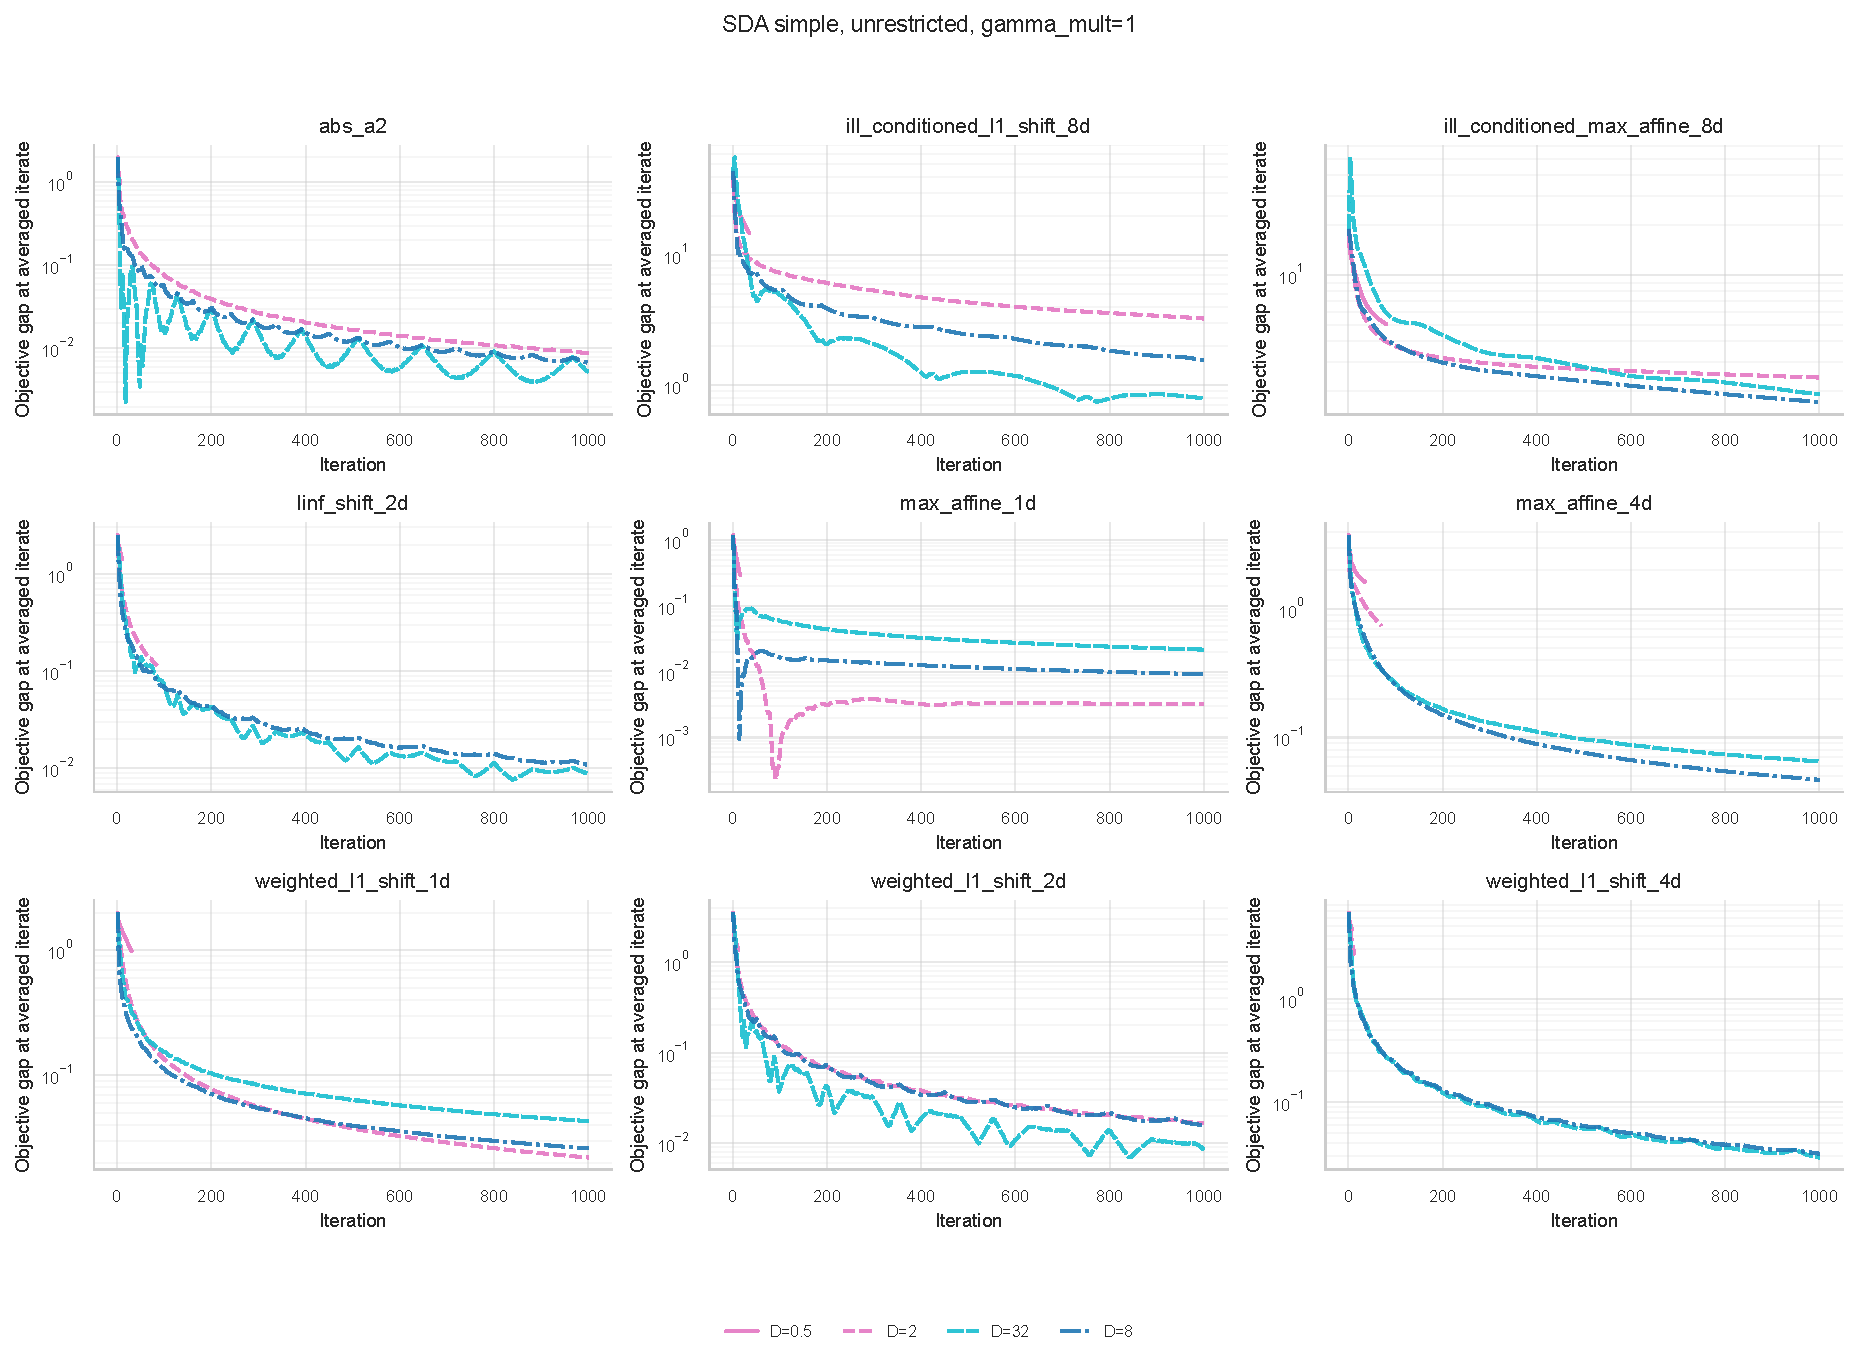
\includegraphics[width=\textwidth]{nonsmooth_objective_grid/nonsmooth_default_unrestricted.pdf}
\caption{Default unrestricted simple Euclidean SDA trajectories.  The plot illustrates that an invalid radius choice can produce a small or negative primal--dual certificate gap while the true objective gap remains large.}
\label{fig:nonsmooth-unrestricted}
\end{figure}

\paragraph{Restricted SDA.}
Figure~\ref{fig:nonsmooth-restricted} repeats the default SDA comparison but
forces the iterates to remain inside \(F_D\).  In this case the algorithm is
solving the restricted problem on the prox ball.  The primal--dual certificate gap is then
consistent with the feasible problem being solved, and the fake early
convergence caused by an invalid primal--dual certificate gap is removed.  The price is that the
optimization problem has changed: the reported solution is a solution for
\(\min_{x\in F_D} f(x)\), not necessarily for the original problem over the
larger ambient set \(Q\).  Thus restriction is useful for illustrating the
radius assumption, but it is less general than applying SDA to the original
problem with prior knowledge that \(x^\star\in F_D\).

\begin{figure}[htbp]
\centering
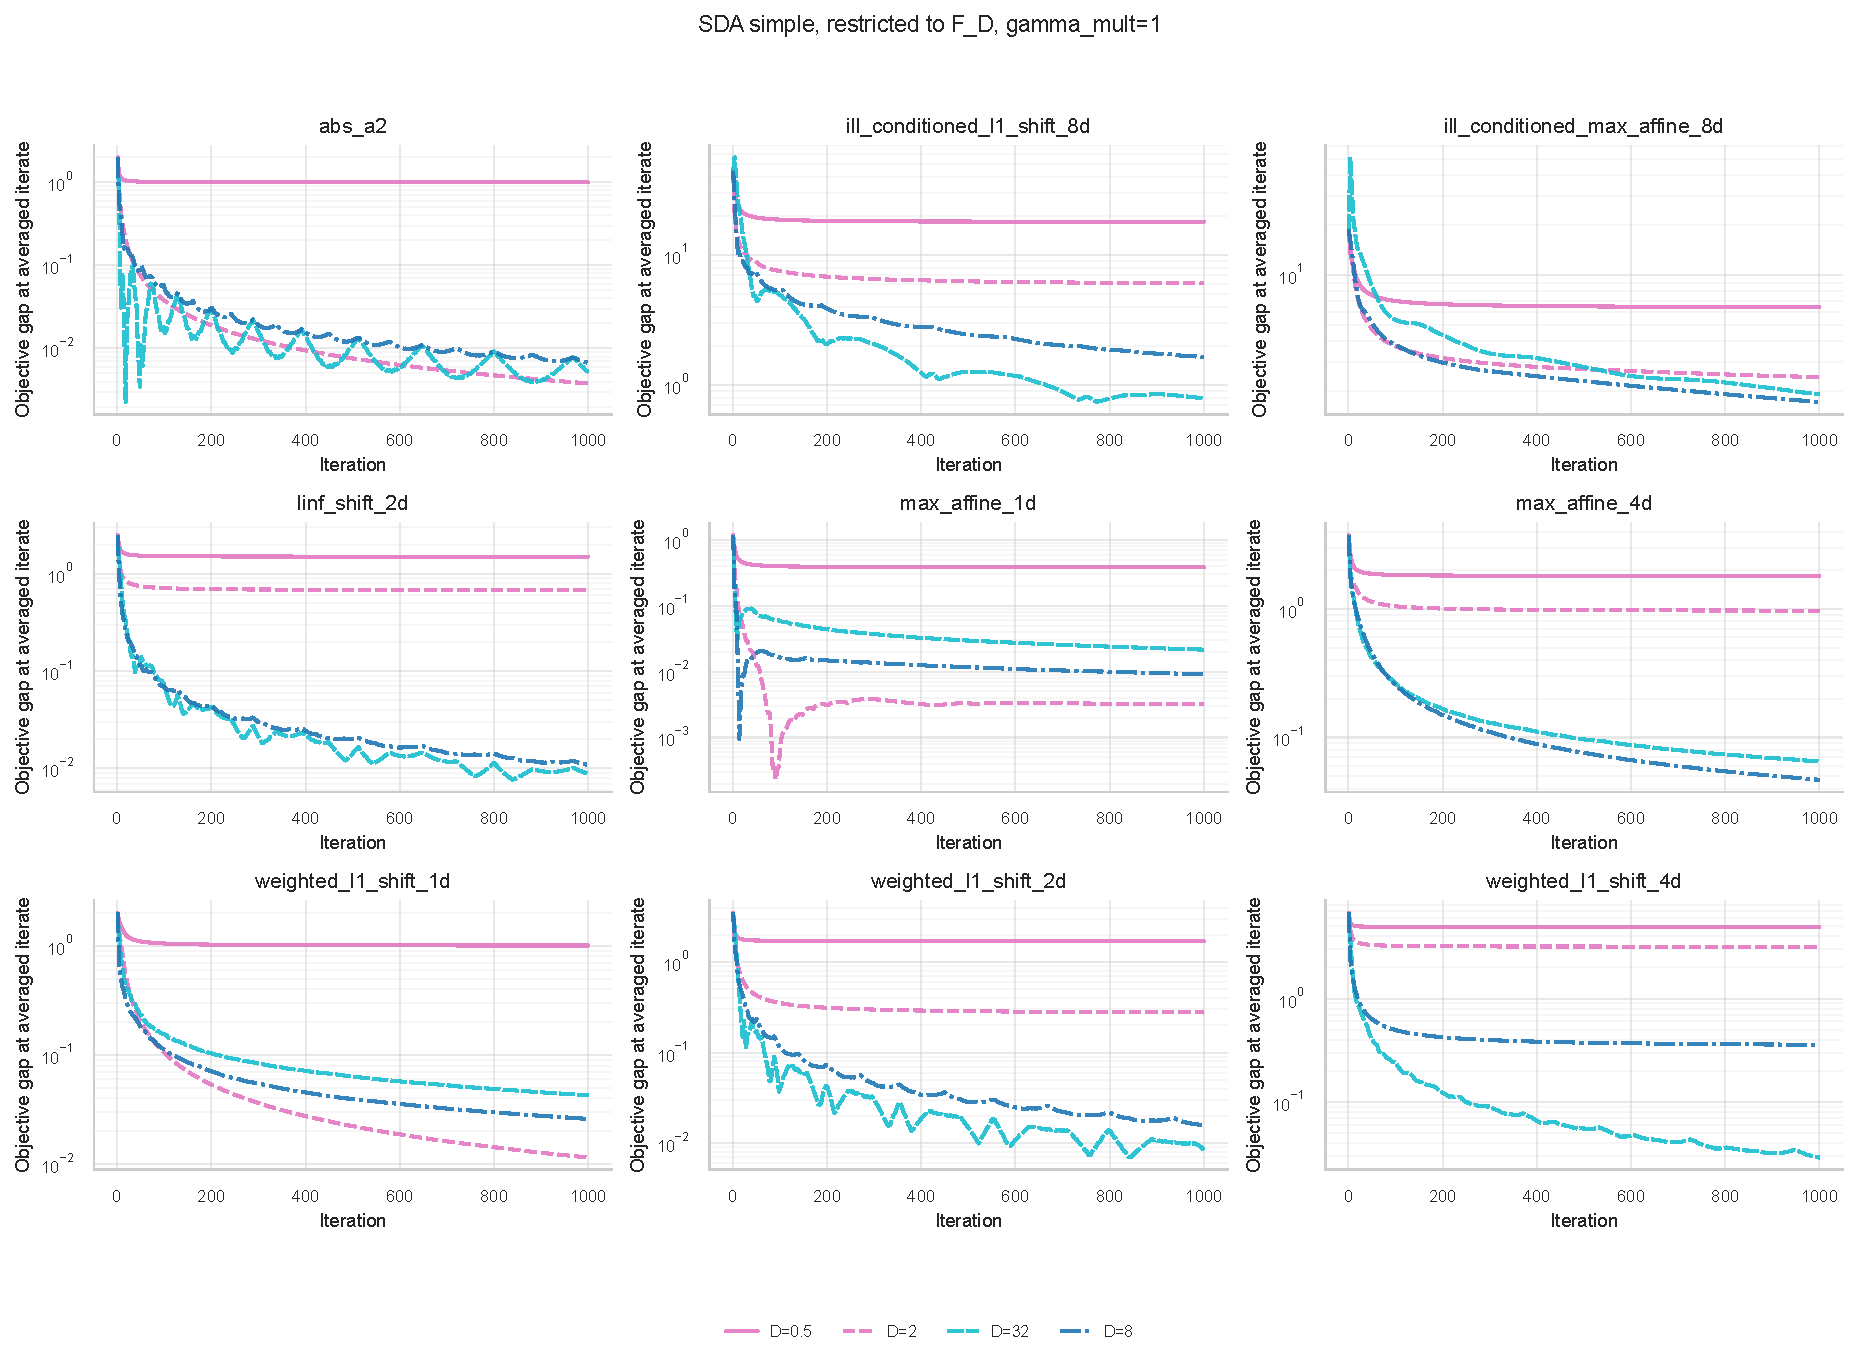
\includegraphics[width=\textwidth]{nonsmooth_objective_grid/nonsmooth_default_restricted.pdf}
\caption{Default restricted simple Euclidean SDA trajectories.  Restricting to \(F_D\) prevents invalid primal--dual-certificate-based stopping, but changes the optimization problem to the prox-ball-restricted problem.}
\label{fig:nonsmooth-restricted}
\end{figure}

Figure~\ref{fig:nonsmooth-restriction-gap} compares unrestricted and restricted
runs more directly.  Even when \(D\) is large enough to contain a minimizer, the
two variants may follow different trajectories.  The unrestricted method can
temporarily move outside \(F_D\) and later return, whereas the restricted method
forbids such movement.  Therefore the restricted variant is not simply a safer
implementation of the same trajectory; it is a different constrained algorithm.
For the remaining benchmark discussion, the unrestricted runs are the main
focus because they represent the intended use of SDA for the original problem.
This interpretation requires external knowledge, or a conservative bound, that
the selected \(D\) contains a minimizer.

\begin{figure}[htbp]
\centering
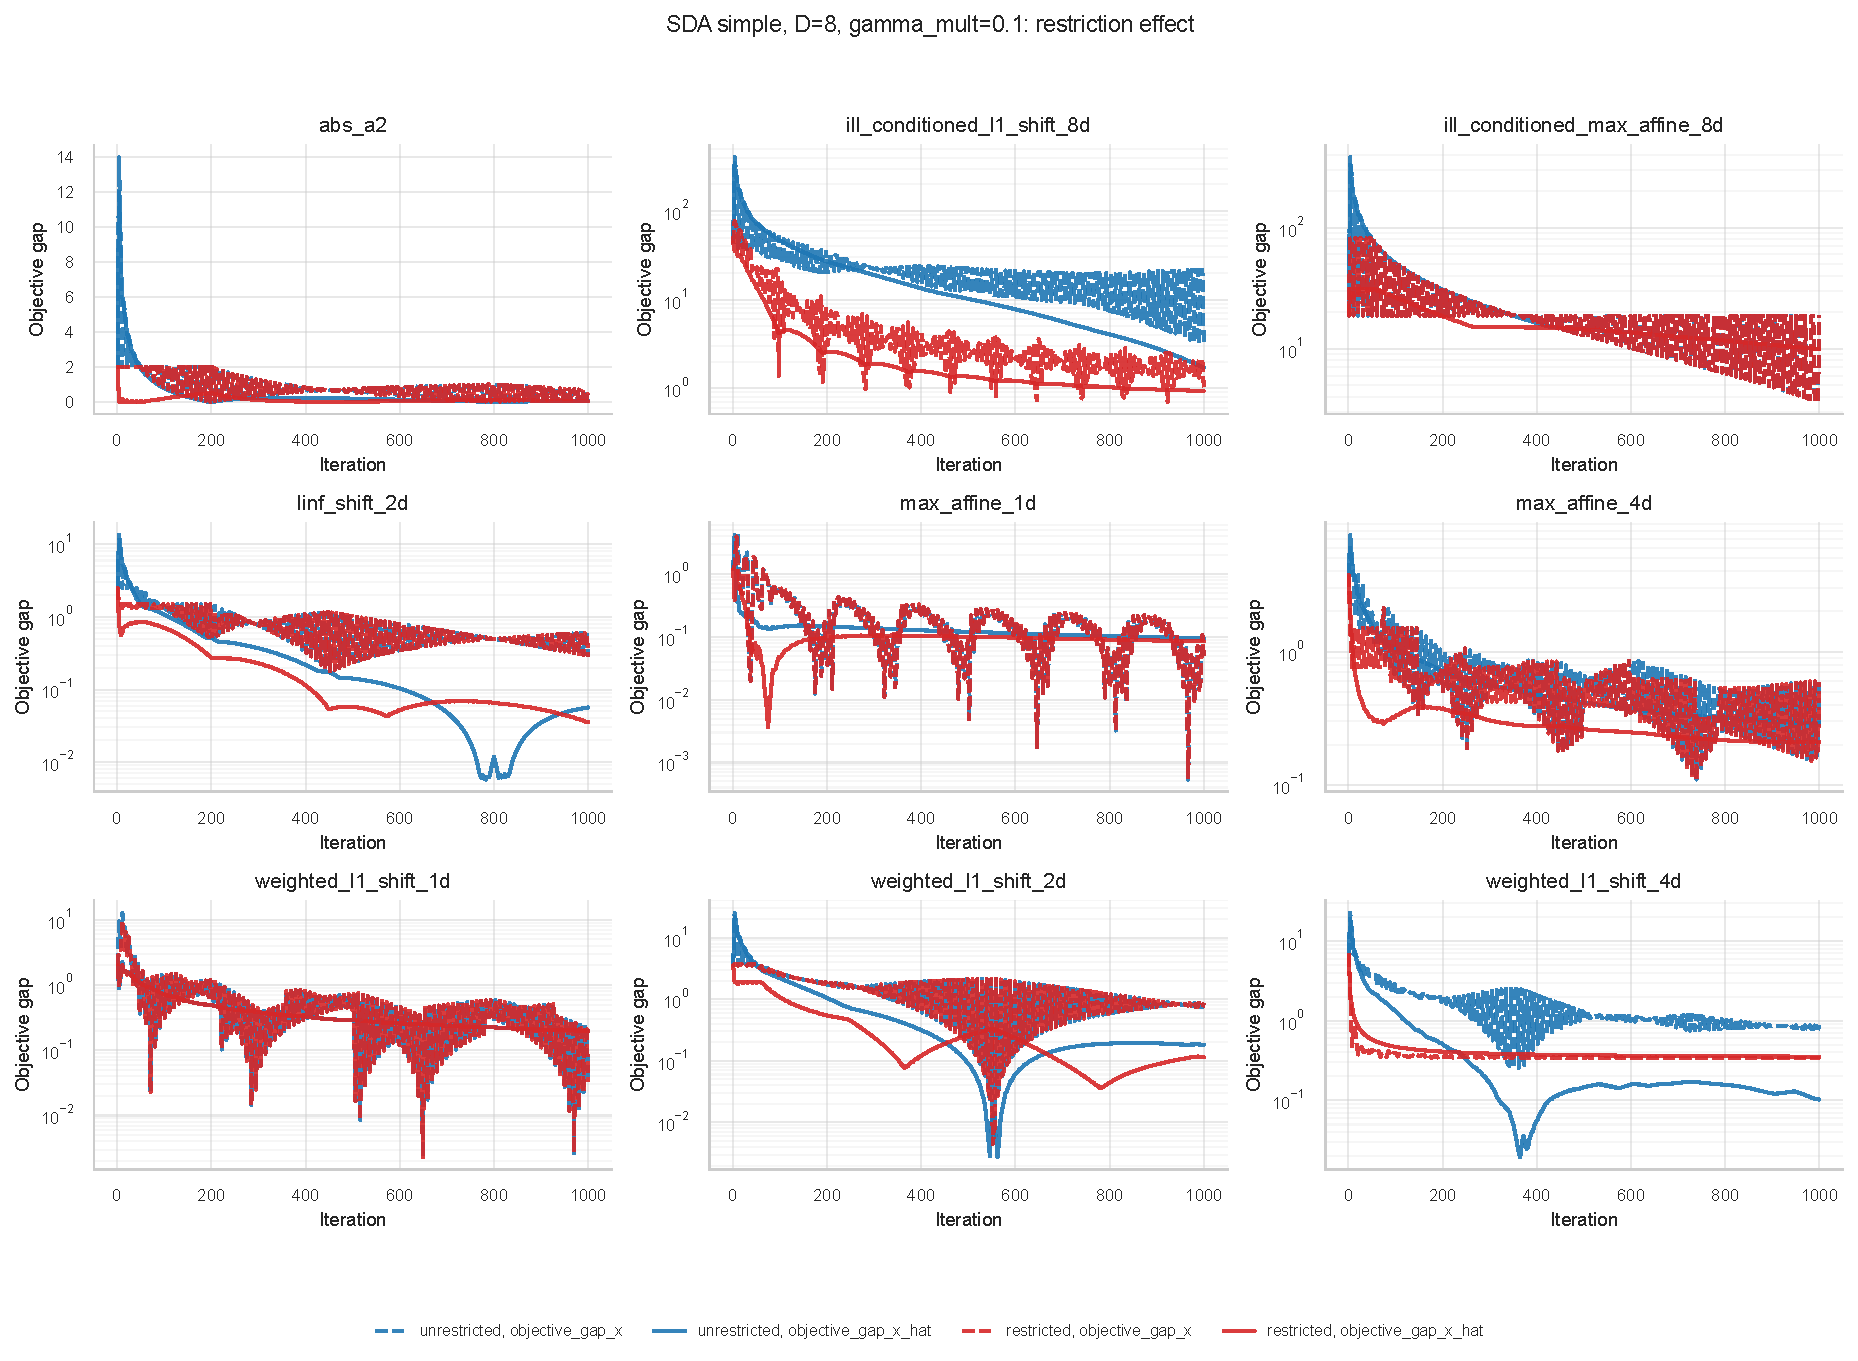
\includegraphics[width=\textwidth]{nonsmooth_objective_grid/nonsmooth_restriction_norm_gap.pdf}
\caption{Current-iterate and averaged-iterate objective gaps for restricted and unrestricted SDA.  The trajectories can differ even when the minimizer lies inside the chosen prox radius.}
\label{fig:nonsmooth-restriction-gap}
\end{figure}

\paragraph{Step-size and radius sensitivity.}
Figure~\ref{fig:nonsmooth-gamma-sweep} fixes \(D=8\) and compares several
\(\gamma_{\mathrm{mult}}\) values.  The implemented step is a multiplier of the Nesterov baseline
step, so \(\gamma_{\mathrm{mult}}=1\) corresponds to the proposed theoretical
scale used by the code.  The parameter \(\gamma\) controls how strongly the
accumulated dual subgradient model affects the next prox-center minimization:
larger values produce more aggressive movement in response to the observed
subgradients, while smaller values produce more conservative movement.  The
figure shows that the baseline multiplier is not always the best empirical
choice in terms of objective-gap decrease.  This is mathematically reasonable:
the theoretical step is based on worst-case bounds, while the benchmark
objectives have different local geometry, subgradient magnitudes, and distances
from the initial point to the minimizer.

\begin{figure}[htbp]
\centering
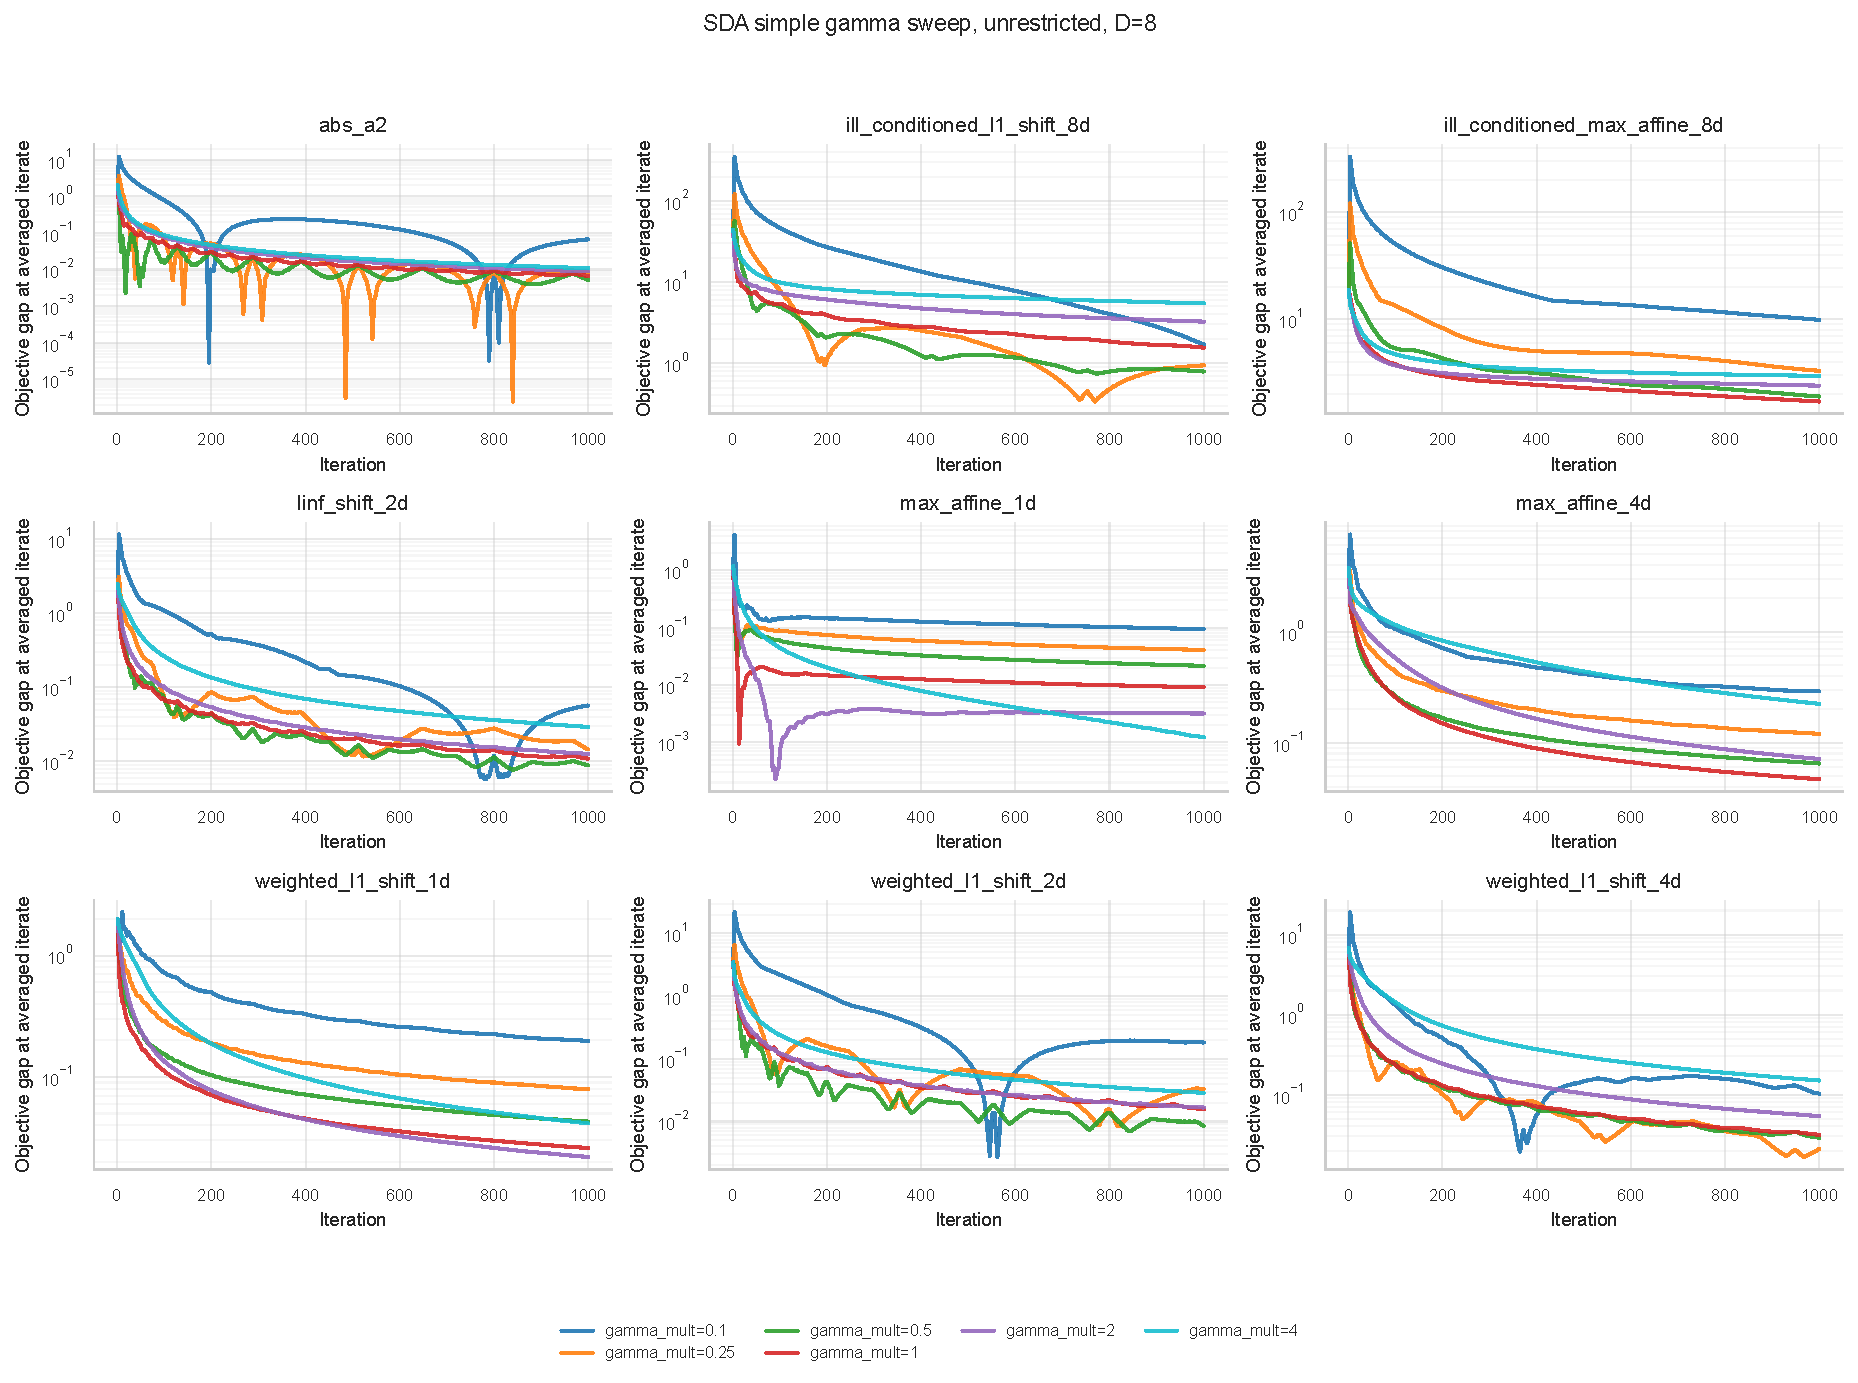
\includegraphics[width=\textwidth]{nonsmooth_objective_grid/nonsmooth_gamma_sweep.pdf}
\caption{Sensitivity of nonsmooth benchmark performance to \(\gamma_{\mathrm{mult}}\) at fixed \(D=8\).  The baseline \(\gamma_{\mathrm{mult}}=1\) is not uniformly optimal.}
\label{fig:nonsmooth-gamma-sweep}
\end{figure}

Figure~\ref{fig:nonsmooth-gamma-d-grid} shows that \(\gamma\) and \(D\) should
be considered jointly.  The radius \(D\) determines the prox ball used in the
primal--dual certificate gap and changes the scale of the theoretical step through the
diameter/radius bound.  The step size determines how quickly the dual aggregate
is translated into primal movement.  If \(D\) is too small, the primal--dual certificate gap may
not apply to the original problem.  If \(D\) is very large, the corresponding
step scale can become too aggressive unless the multiplier is adjusted.  Thus a
multiplier that is effective for one radius may be poor for another radius.  In
practice, \(D\) should be chosen from prior knowledge or a conservative bound on
the solution radius, and \(\gamma_{\mathrm{mult}}\) should be tuned relative to
that choice.

\begin{figure}[htbp]
\centering
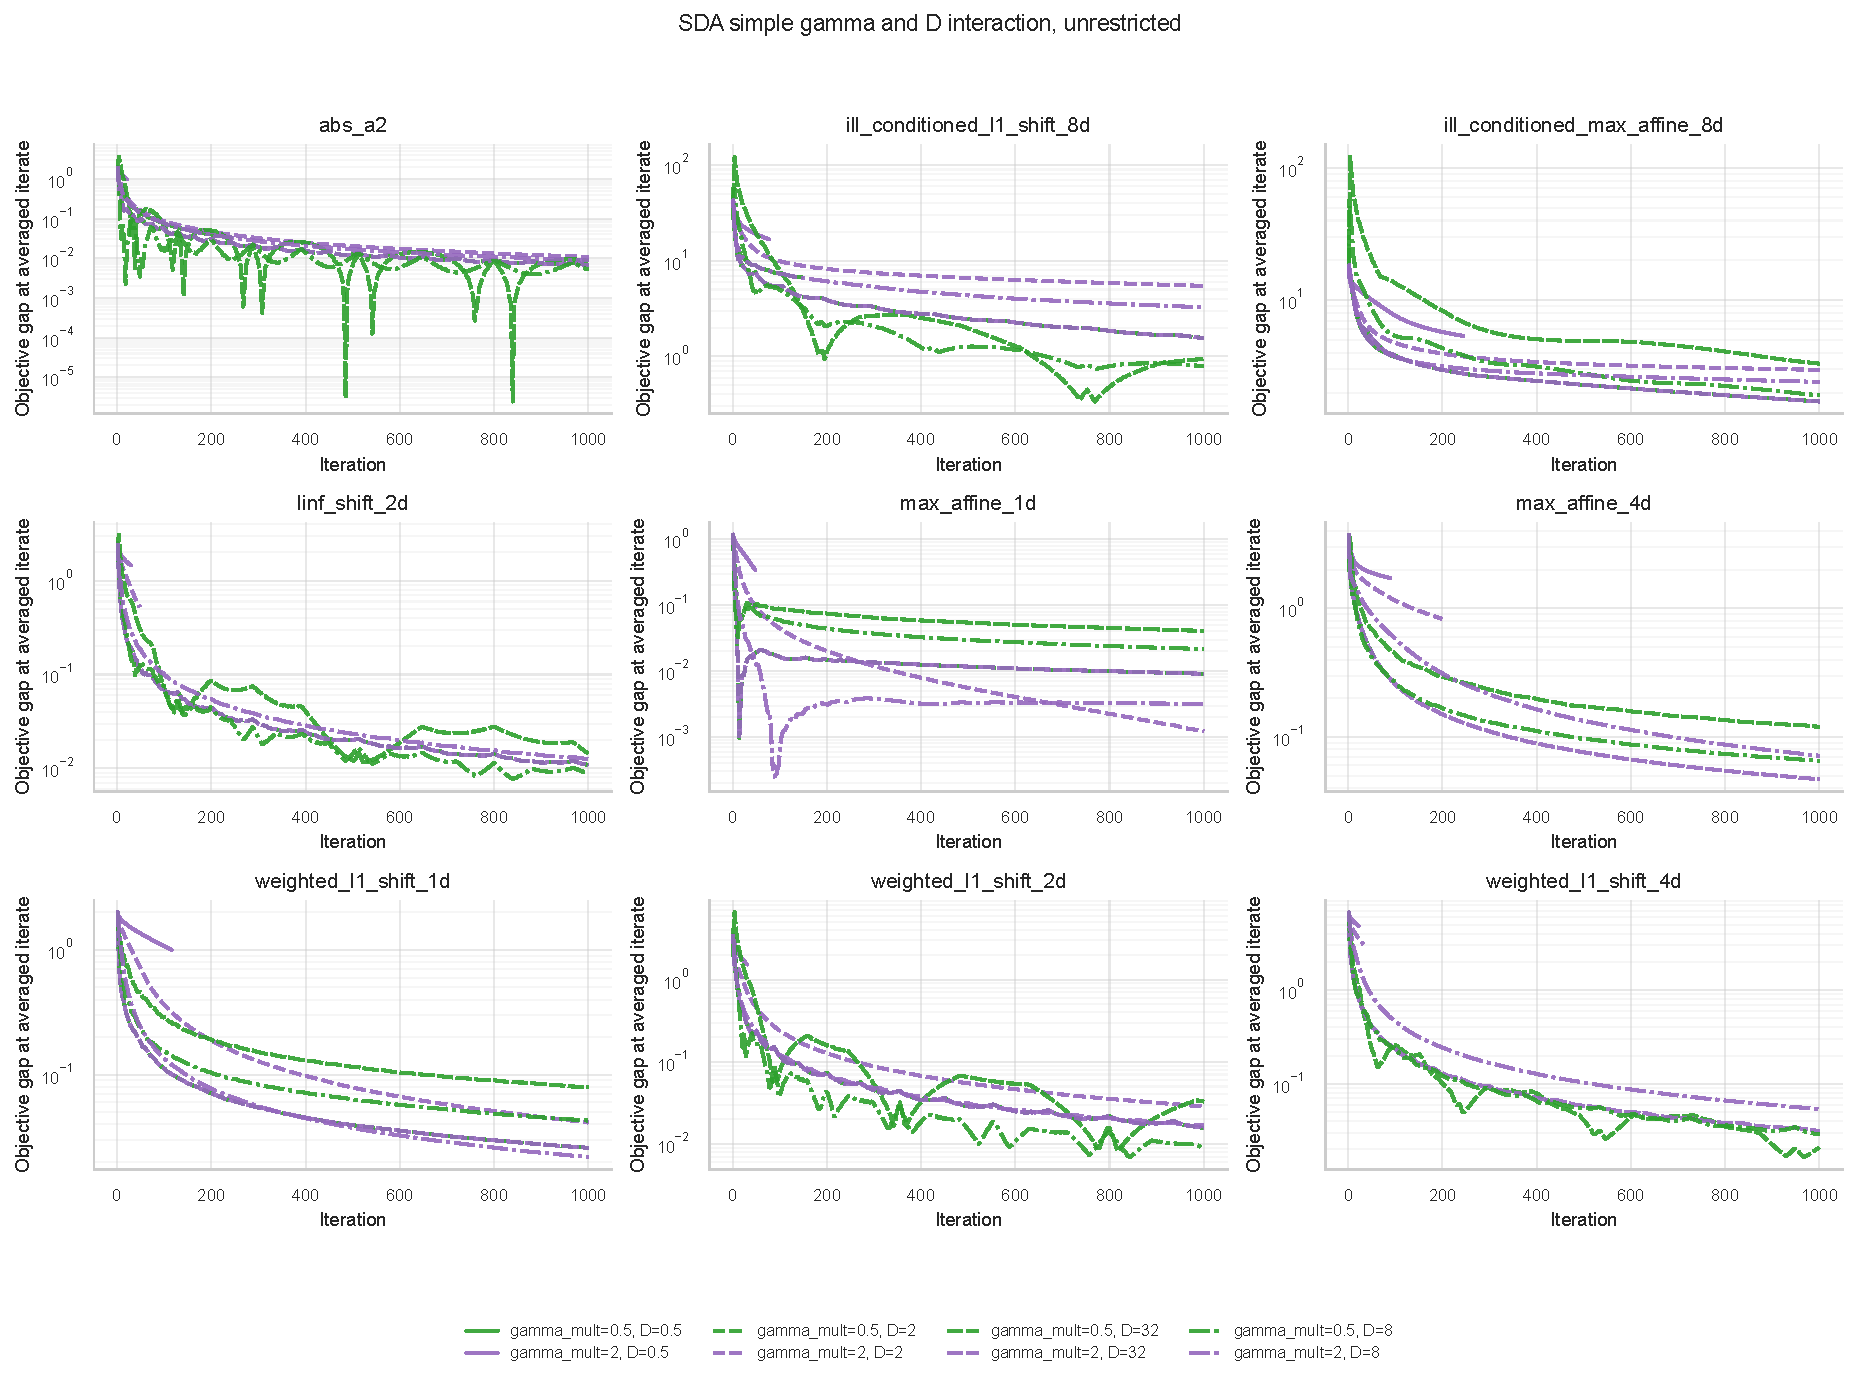
\includegraphics[width=\textwidth]{nonsmooth_objective_grid/nonsmooth_gamma_d_grid.pdf}
\caption{Interaction between prox-radius parameter \(D\) and step multiplier \(\gamma_{\mathrm{mult}}\).  The useful parameter is the pair \((D,\gamma_{\mathrm{mult}})\), not either value in isolation.}
\label{fig:nonsmooth-gamma-d-grid}
\end{figure}

\paragraph{Method comparison.}
Figures~\ref{fig:nonsmooth-methods} and \ref{fig:nonsmooth-runtime} compare
simple SDA, weighted SDA, and projected subgradient descent.  On these
benchmark functions, the standard projected subgradient method can behave as
well as, or better than, SDA for several objectives, and it is usually faster in
wall-clock time.  Table~\ref{tab:nonsmooth-summary} reflects this: projected
subgradient has the smallest median final objective gap over the full nonsmooth grid,
while the best single run is achieved by weighted SDA.  This should not be
interpreted as a contradiction of SDA theory.  The methods solve slightly
different algorithmic subproblems, the grid includes invalid small-radius SDA
runs, and the theoretical guarantees are worst-case bounds rather than
predictions of dominance on every small benchmark.

The runtime plot also clarifies why final objective gaps must be read together with the
radius condition.  Some SDA points with very small runtime and large true
objective gap correspond to runs that stopped early because \(D\) was too small
and the computed primal--dual certificate gap became invalid or negative.  These are not
successful fast convergences.  They are examples of the fake convergence
mechanism shown in Figure~\ref{fig:nonsmooth-unrestricted}.

\begin{figure}[htbp]
\centering
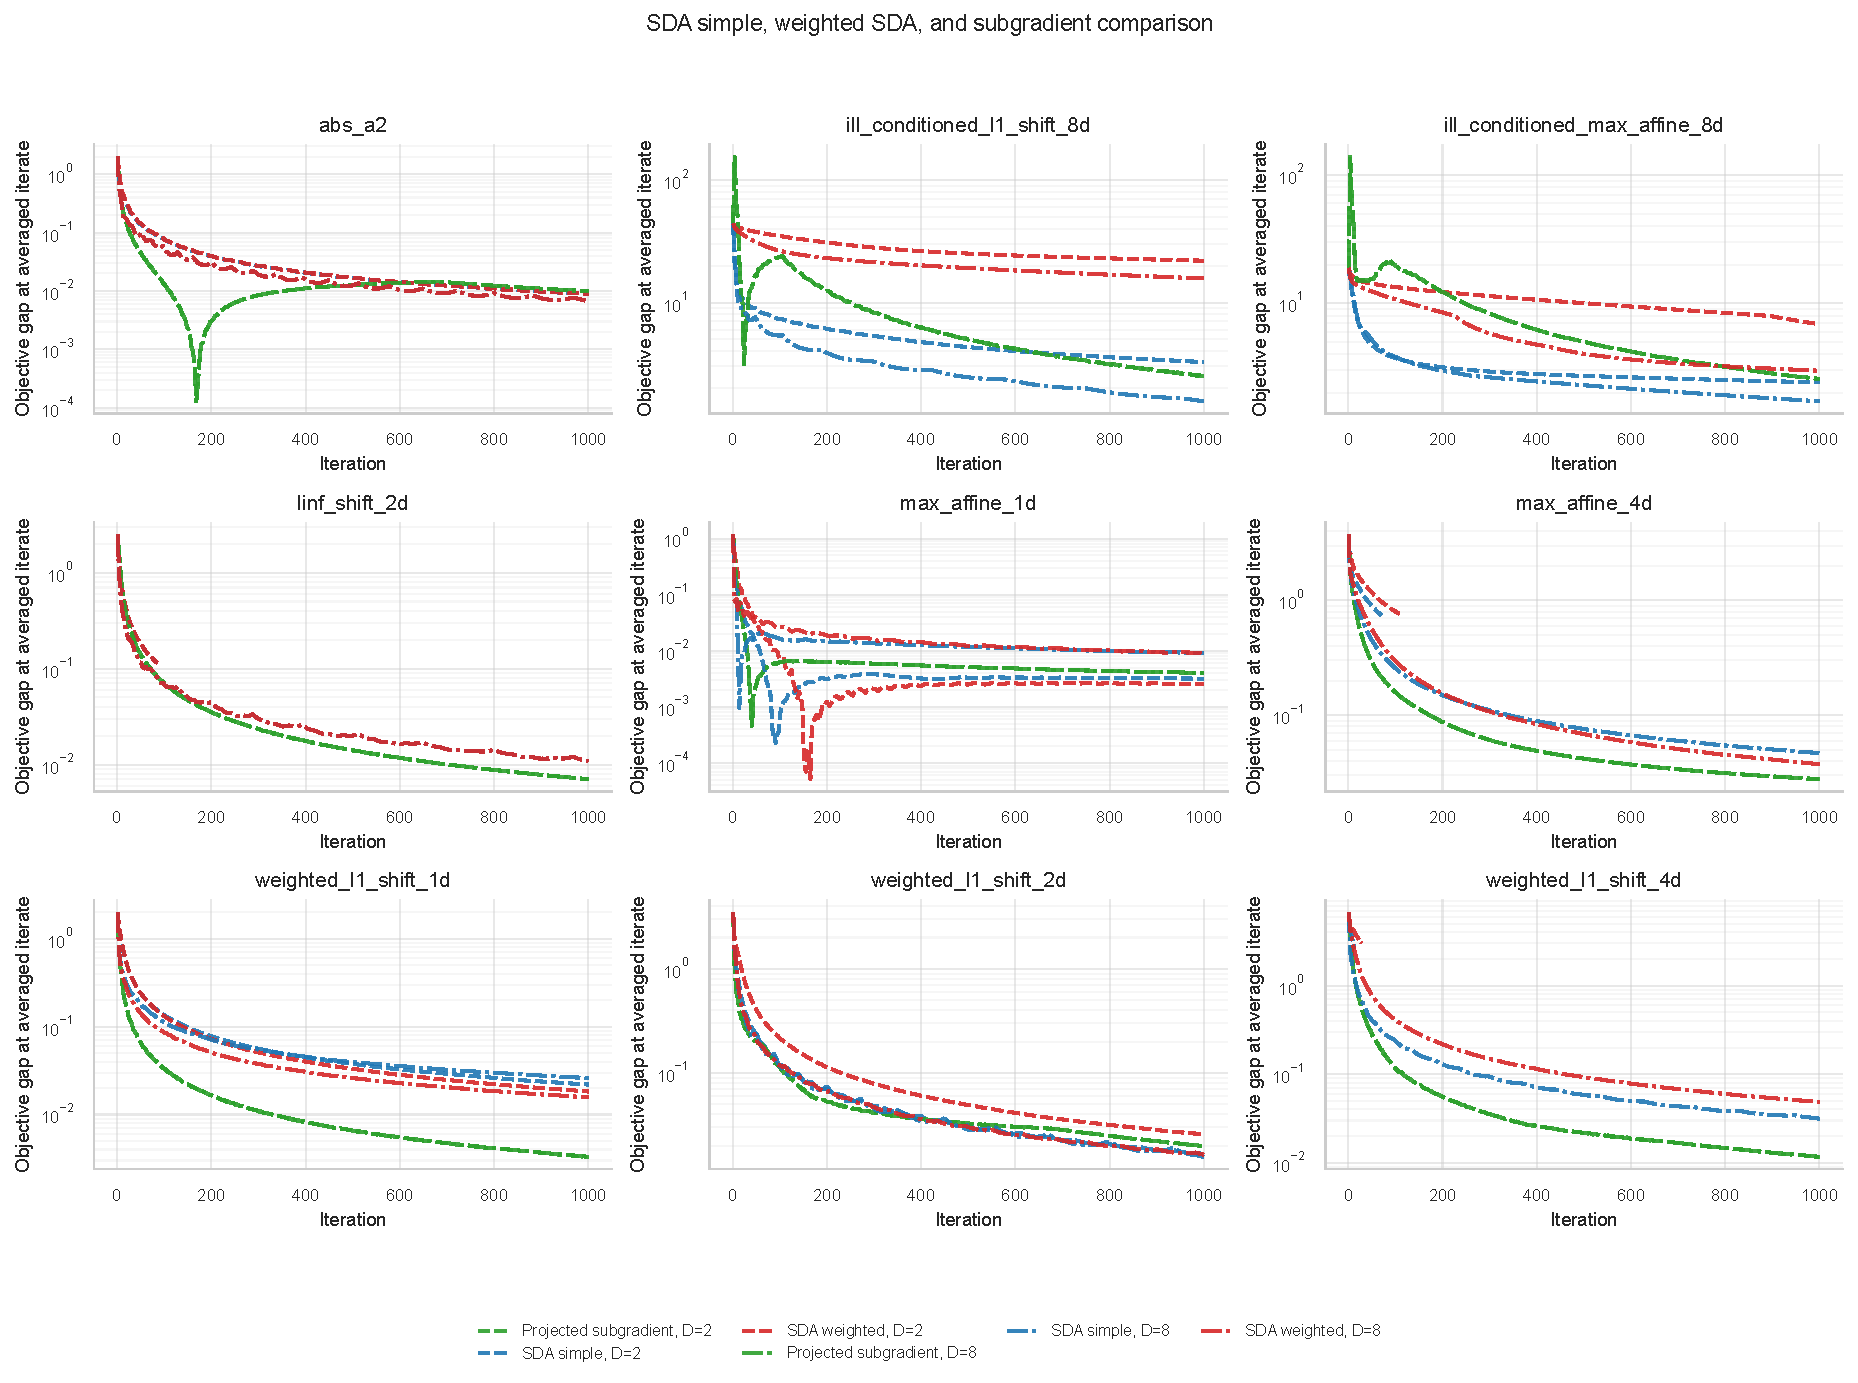
\includegraphics[width=\textwidth]{nonsmooth_objective_grid/nonsmooth_method_comparison.pdf}
\caption{Default comparison of simple SDA, weighted SDA, and projected subgradient descent on nonsmooth benchmark objectives.}
\label{fig:nonsmooth-methods}
\end{figure}

\begin{figure}[htbp]
\centering
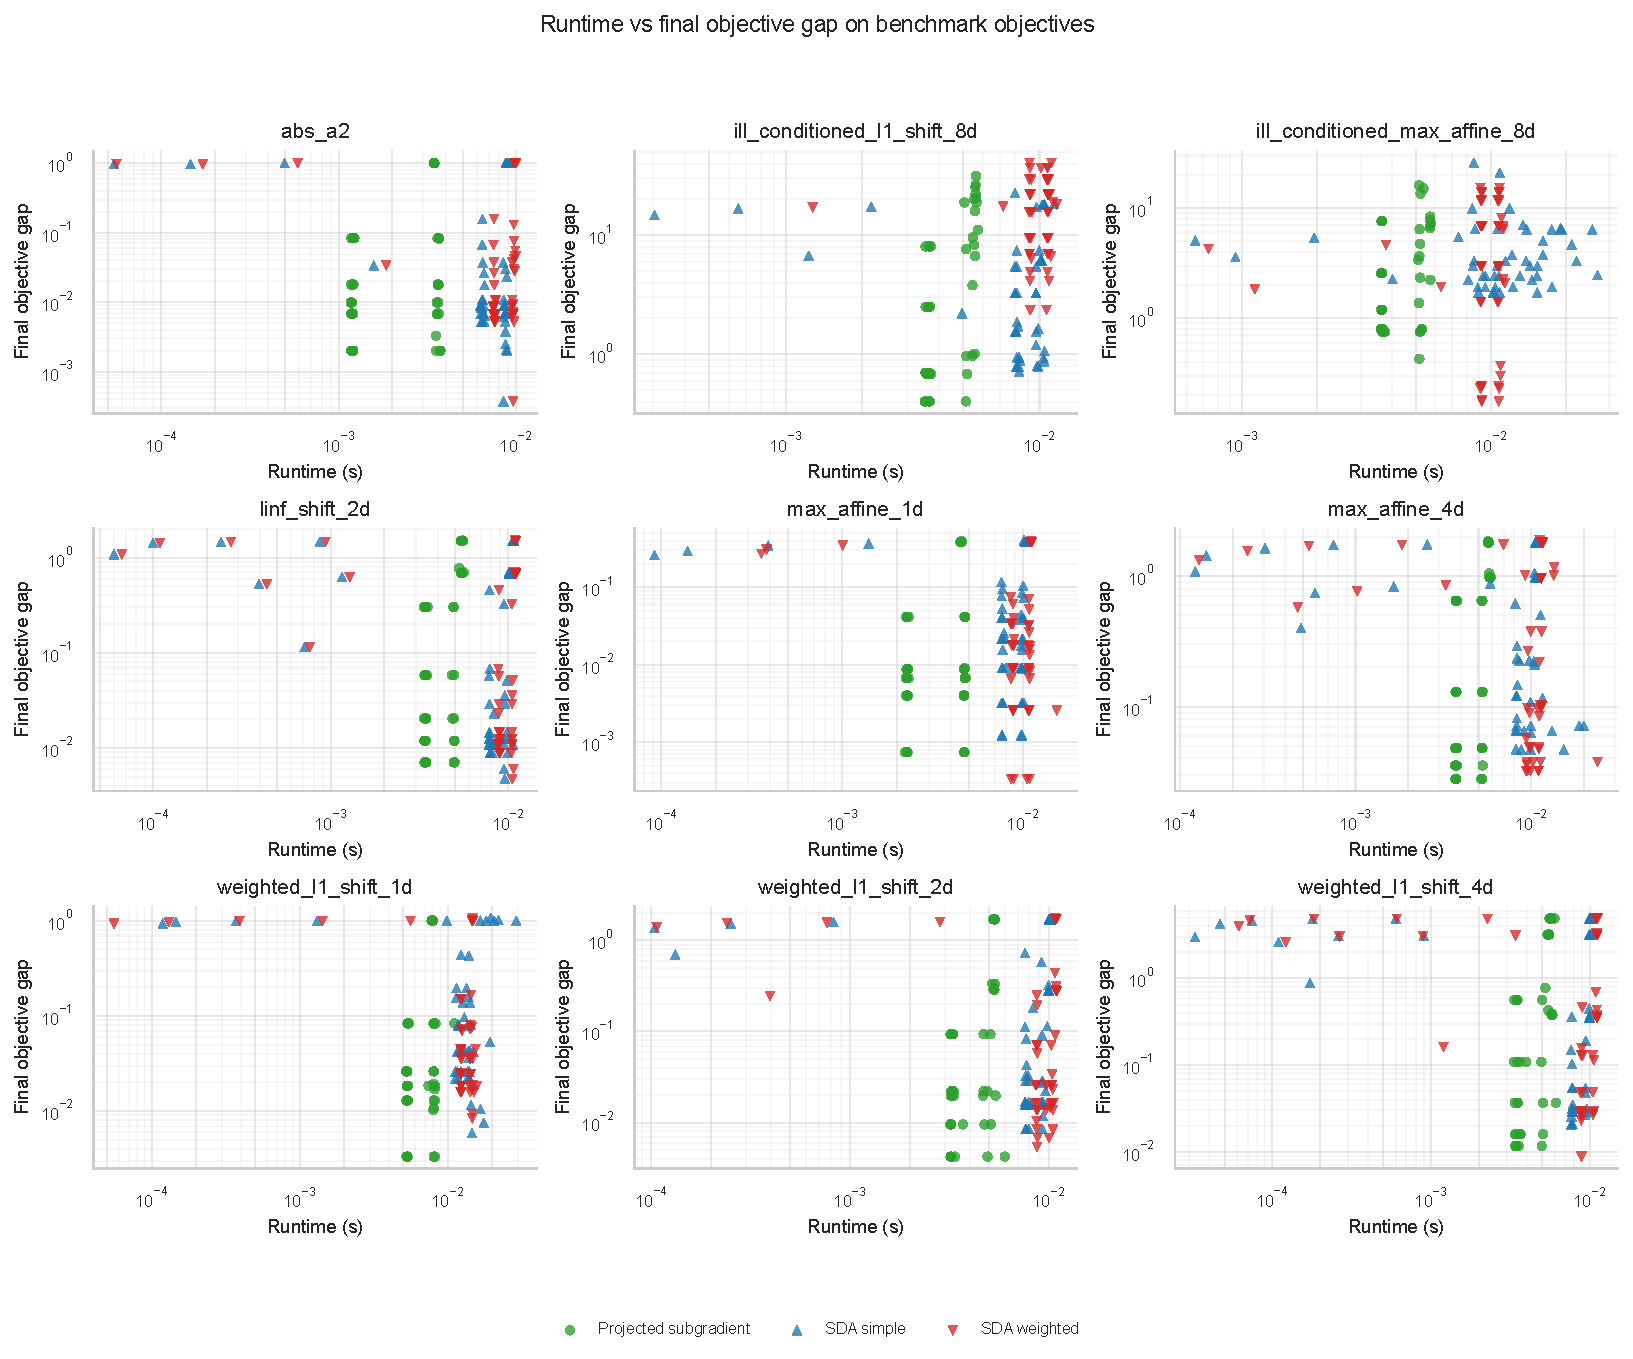
\includegraphics[width=\textwidth]{nonsmooth_objective_grid/nonsmooth_runtime_vs_final_objective_gap.pdf}
\caption{Runtime versus final true objective gap for nonsmooth benchmark objectives.  Low-runtime, high-objective-gap SDA points are often invalid early stops caused by too small a radius.}
\label{fig:nonsmooth-runtime}
\end{figure}

\FloatBarrier

\subsection{Prox Geometry Comparison}
\label{subsec:prox-geometry}

\paragraph{Purpose and setup.}
The second experiment isolates the effect of the prox geometry.  It uses three
coordinate-imbalanced nonsmooth objectives: an ill-conditioned shifted
\(\ell_1\) objective, an ill-conditioned max-affine objective, and a weighted
\(\ell_1\) objective.  The methods are Euclidean SDA and weighted Euclidean
SDA, each with simple and weighted dual averaging.  For the weighted Euclidean
prox, three diagonal profiles are tested: uniform, coordinate-matched, and
inverse-coordinate-matched.  The grid uses
\(D\in\{2,8,32\}\), \(\gamma_{\mathrm{mult}}\in\{0.5,1,2\}\), and both
restricted and unrestricted runs, for 432 runs total.

\begin{table}[htbp]
\centering
\small
\resizebox{\textwidth}{!}{%
\begin{tabular}{lrrrr}
\toprule
Method & Runs & Median final objective gap & Best objective gap & Median runtime (s) \\
\midrule
SDA simple, Euclidean prox & 54 & \(1.36\) & \(1.24\cdot 10^{-2}\) & \(1.45\cdot 10^{-2}\) \\
SDA simple, weighted prox & 162 & \(2.18\) & \(1.24\cdot 10^{-2}\) & \(1.60\cdot 10^{-2}\) \\
SDA weighted, Euclidean prox & 54 & \(3.14\) & \(1.94\cdot 10^{-2}\) & \(1.51\cdot 10^{-2}\) \\
SDA weighted, weighted prox & 162 & \(2.92\) & \(1.94\cdot 10^{-2}\) & \(1.89\cdot 10^{-2}\) \\
\bottomrule
\end{tabular}
}
\caption{Aggregate final objective gaps \(f(\hat x)-f^\star\) in the prox-geometry experiment.}
\label{tab:prox-summary}
\end{table}

Figure~\ref{fig:prox-geometry} shows that diagonal geometry is not uniformly
beneficial.  The coordinate-matched profile can improve behavior on objectives
whose anisotropy agrees with that profile, but the inverse profile is a useful
negative control: it emphasizes the wrong coordinates and may slow convergence.
This is consistent with mirror-descent intuition.  A prox function improves a
method only when it represents the geometry of the feasible set and the
subgradients well; an arbitrary change of norm is not a free acceleration.

\begin{figure}[htbp]
\centering
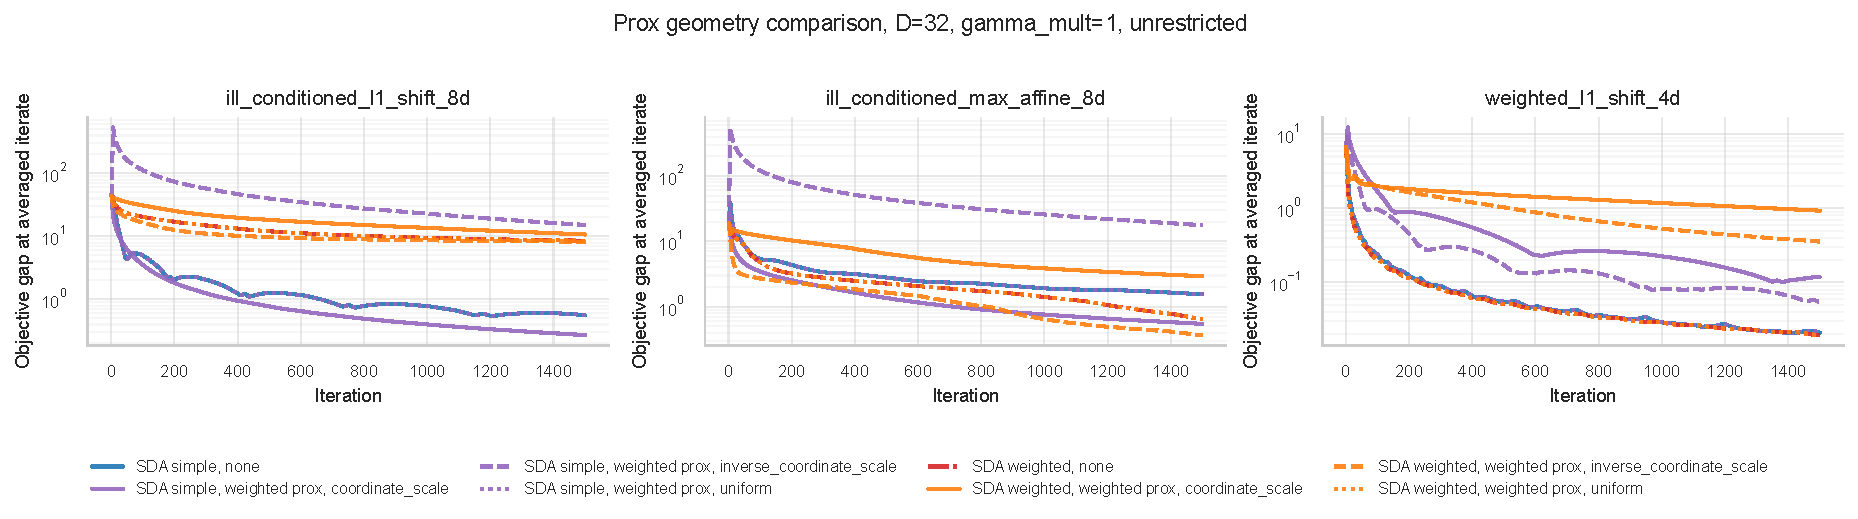
\includegraphics[width=\textwidth]{prox_geometry_comparison/prox_geometry.pdf}
\caption{Euclidean and weighted Euclidean prox choices on coordinate-imbalanced objectives.}
\label{fig:prox-geometry}
\end{figure}

The runtime summary in Figure~\ref{fig:prox-runtime} leads to the same
conclusion.  Weighted geometry introduces a small additional computational cost
in these low-dimensional tests, and its optimization benefit depends on the
objective.  The median objective gaps in Table~\ref{tab:prox-summary} are therefore best
read together with the per-objective panels rather than as an absolute ranking
of all geometries.

\begin{figure}[htbp]
\centering
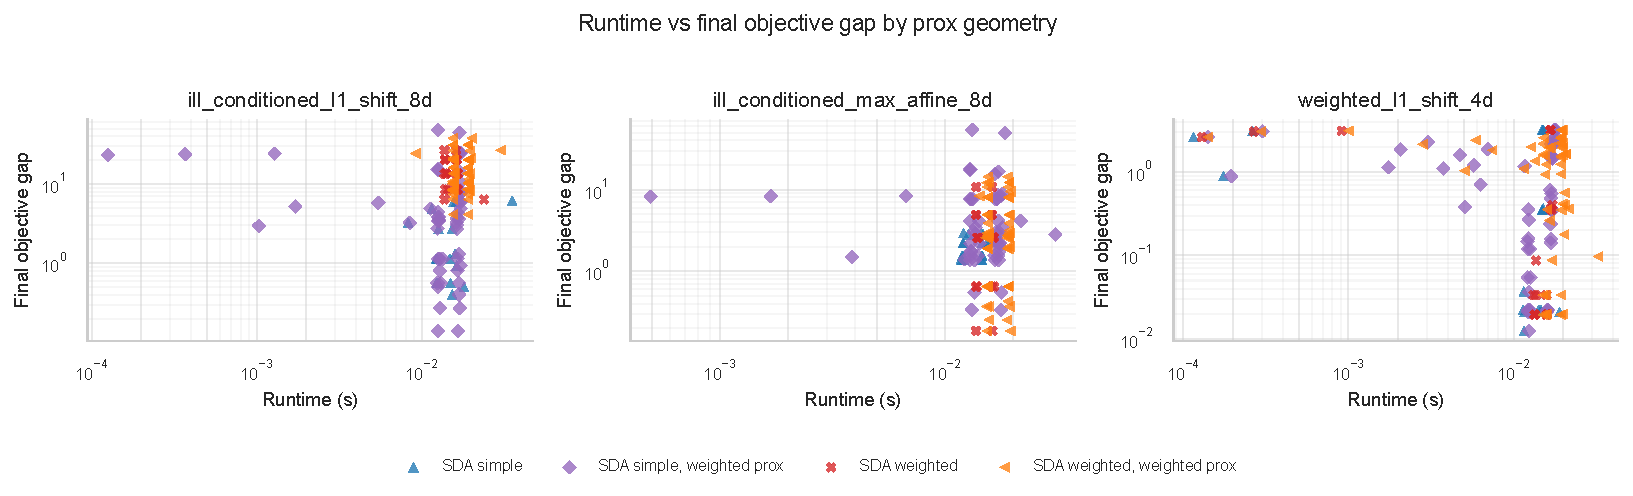
\includegraphics[width=\textwidth]{prox_geometry_comparison/prox_runtime_vs_final_objective_gap.pdf}
\caption{Runtime versus final true objective gap for prox-geometry runs.}
\label{fig:prox-runtime}
\end{figure}

\FloatBarrier

\subsection{Entropy Geometry on Simplex Objectives}
\label{subsec:simplex}

\paragraph{Purpose and setup.}
The third experiment tests entropy prox on simplex-constrained objectives.  The
simplex is a natural setting for entropy geometry because the primal geometry is
\(\ell_1\)-like and the dual norm is \(\ell_\infty\).  The objectives are
\texttt{simplex\_linear\_8d}, \texttt{simplex\_max\_affine\_8d}, and
\texttt{simplex\_sparse\_max\_affine\_16d}.  Simple and weighted entropy SDA
are run with \(D\in\{1,2,3\}\) and
\(\gamma_{\mathrm{mult}}\in\{0.1,0.5,1,4\}\), for 72 runs total.

\begin{table}[htbp]
\centering
\small
\resizebox{\textwidth}{!}{%
\begin{tabular}{lrrrr}
\toprule
Method & Runs & Median final objective gap & Best objective gap & Median runtime (s) \\
\midrule
Entropy SDA simple & 36 & \(8.37\cdot 10^{-3}\) & \(1.09\cdot 10^{-3}\) & \(6.16\cdot 10^{-1}\) \\
Entropy SDA weighted & 36 & \(8.13\cdot 10^{-3}\) & \(1.09\cdot 10^{-3}\) & \(6.57\cdot 10^{-1}\) \\
\bottomrule
\end{tabular}
}
\caption{Aggregate final objective gaps \(f(\hat x)-f^\star\) for entropy prox on simplex objectives.}
\label{tab:simplex-summary}
\end{table}

Figure~\ref{fig:simplex-entropy} shows that the simple and weighted entropy
variants are close in median final objective gap.  The best run on
\texttt{simplex\_linear\_8d} is achieved by simple entropy SDA with
\(D=3\) and \(\gamma_{\mathrm{mult}}=0.1\), while the sparse max-affine
objective favors the weighted entropy variant in the best run.  This supports a
moderate conclusion: entropy is appropriate for the simplex constraint, but the
weighted averaging rule is not uniformly dominant on these three objectives.

\begin{figure}[htbp]
\centering
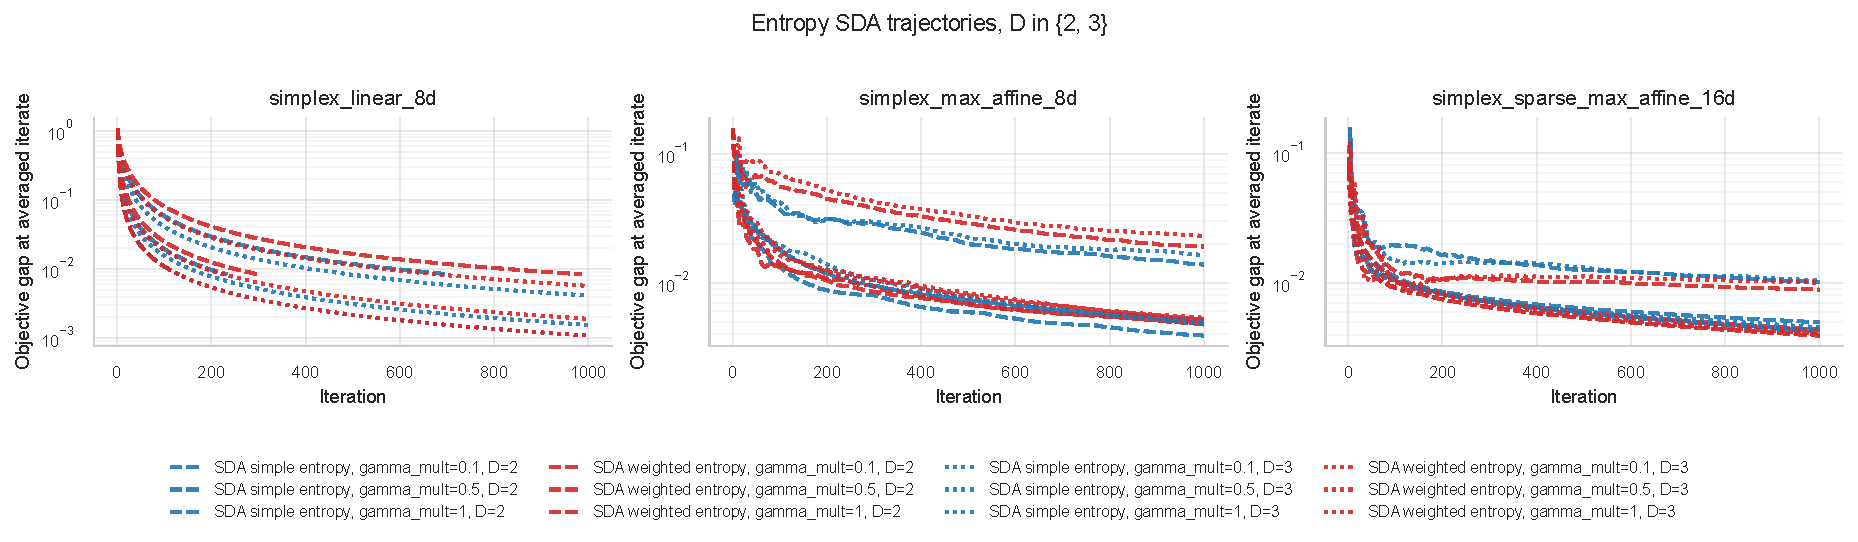
\includegraphics[width=\textwidth]{simplex_entropy_geometry/simplex_entropy.pdf}
\caption{Simple and weighted entropy SDA on simplex-constrained objectives.}
\label{fig:simplex-entropy}
\end{figure}

Figure~\ref{fig:simplex-runtime} shows that the entropy runs are slower than the
small Euclidean benchmark runs, with median runtimes around \(0.6\) seconds.
That runtime reflects the current implementation and the denser simplex
projection/prox computations; it should not be interpreted as a lower bound on
entropy mirror descent.

\begin{figure}[htbp]
\centering
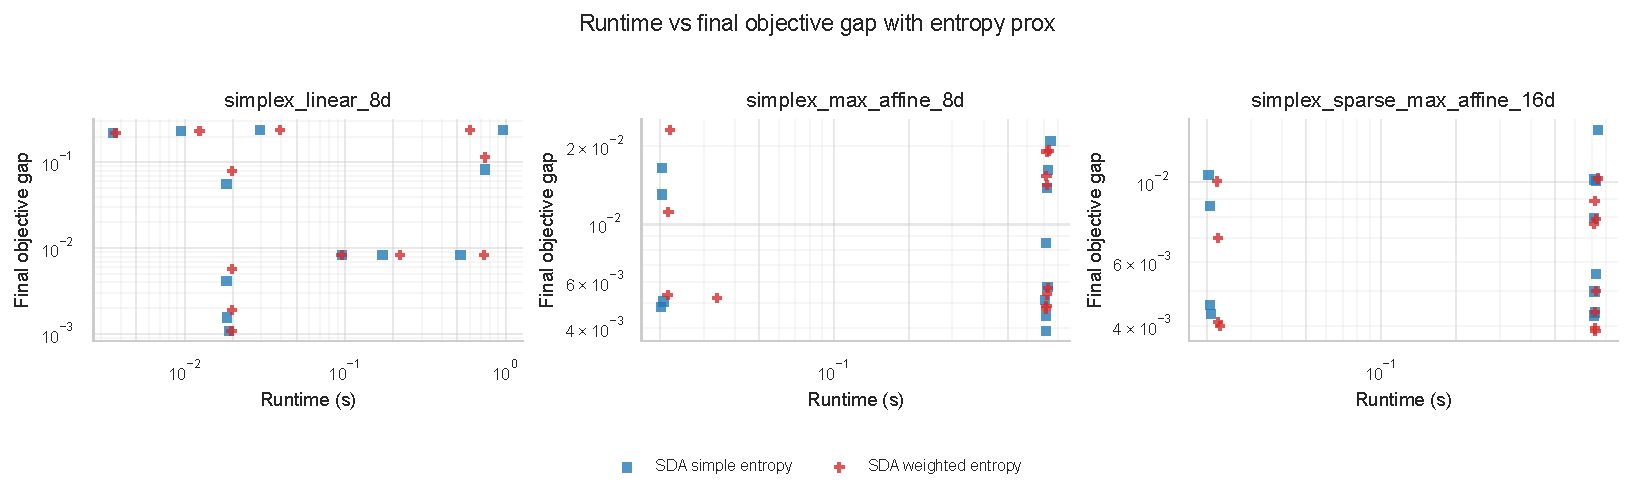
\includegraphics[width=\textwidth]{simplex_entropy_geometry/simplex_runtime_vs_final_objective_gap.pdf}
\caption{Runtime versus final true objective gap for entropy-prox simplex runs.}
\label{fig:simplex-runtime}
\end{figure}

\FloatBarrier

\subsection{Lasso Logistic Sparsity}
\label{subsec:lasso}

\paragraph{Purpose and setup.}
The fourth experiment evaluates the methods on binary lasso logistic regression
datasets.  The objective has the form
\[
    F(w,b)=\frac{1}{n}\sum_{i=1}^n
    \log\!\bigl(1+\exp(x_i^\top w+b)\bigr)-y_i(x_i^\top w+b)
    +\frac{\lambda}{n}\|w\|_1 ,
\]
where the intercept is not penalized.  The current grid uses \(\lambda=1\),
unrestricted iterates, seed \(0\), and a train/test split of \(0.8/0.2\).
The datasets are \texttt{iris}, four synthetic logistic datasets,
\texttt{breast\_cancer\_wdbc}, \texttt{banknote\_authentication}, and
\texttt{spambase}.  The custom methods are simple SDA, weighted SDA, and
projected subgradient; sklearn SAGA is included as the empirical reference.

\begin{table}[htbp]
\centering
\small
\resizebox{\textwidth}{!}{%
\begin{tabular}{lrrrrr}
\toprule
Method & Runs & Median train-objective gap to SAGA & Best train-objective gap & Median runtime (s) & Median accuracy \\
\midrule
Projected subgradient & 72 & \(3.38\cdot 10^{-2}\) & \(4.02\cdot 10^{-4}\) & \(3.60\cdot 10^{-2}\) & \(0.878\) \\
SDA simple & 96 & \(2.03\cdot 10^{-2}\) & \(6.26\cdot 10^{-5}\) & \(4.29\cdot 10^{-2}\) & \(0.878\) \\
SDA weighted & 96 & \(1.74\cdot 10^{-5}\) & \(-1.43\cdot 10^{-3}\) & \(3.87\cdot 10^{-2}\) & \(0.888\) \\
sklearn SAGA & 8 & \(0\) & \(0\) & \(3.75\cdot 10^{-3}\) & \(0.888\) \\
\bottomrule
\end{tabular}
}
\caption{Lasso logistic final train-objective gaps to the matched sklearn SAGA reference.}
\label{tab:lasso-summary}
\end{table}

Figure~\ref{fig:lasso-d} compares the methods over \(D\).  Weighted SDA is the
most reliable method in this lasso grid: it has the smallest median train-objective gap to the
SAGA reference and is the best custom method on every dataset in the final-run
CSV.  This is a statement about this parameter grid, not a general theorem.
The lasso objective is convex but nonsmooth because of the \(\ell_1\) term, and
the experiment uses subgradients of the penalty rather than the exact proximal
regularized dual averaging update studied by Xiao \cite{xiao_regularized_dual_averaging}.

\begin{figure}[htbp]
\centering
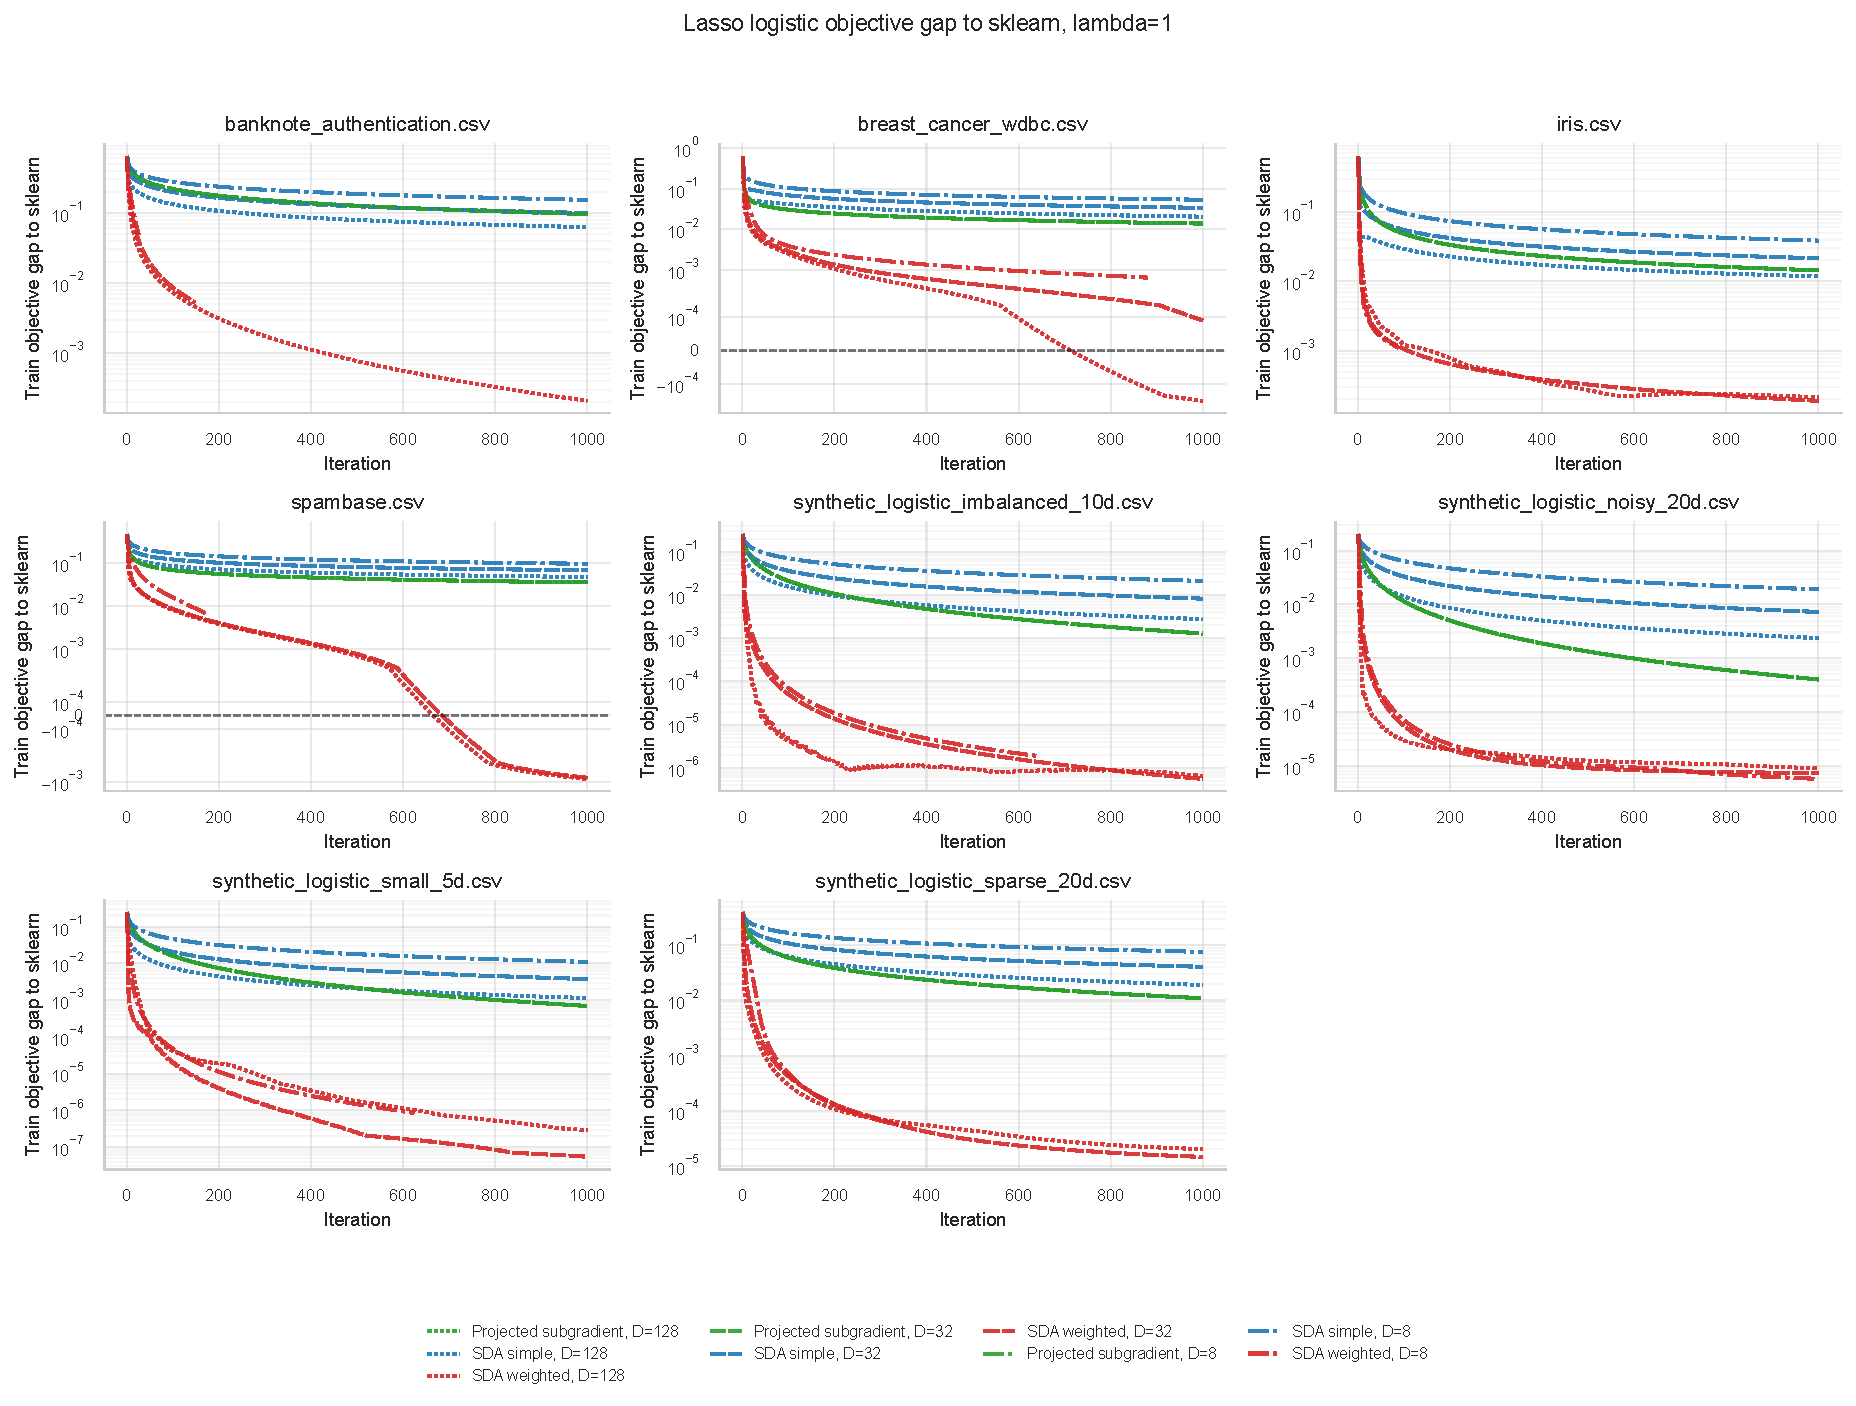
\includegraphics[width=\textwidth]{lasso_logistic_sparsity/lasso_d_comparison.pdf}
\caption{Effect of \(D\) on lasso logistic train-objective gap to the sklearn SAGA reference.}
\label{fig:lasso-d}
\end{figure}

Figure~\ref{fig:lasso-param} fixes \(D=32\) and varies the SDA multiplier
\(\gamma_{\mathrm{mult}}\) or projected-subgradient step \(\alpha\).  The
parameter sensitivity is substantial: a method that is competitive at one step
scale can be much worse at another.  The absolute train-objective view in
Figure~\ref{fig:lasso-train} confirms that the smallest train-objective gaps correspond to
curves approaching the matched SAGA train objective, rather than to an artifact
of plotting only differences.

\begin{figure}[htbp]
\centering
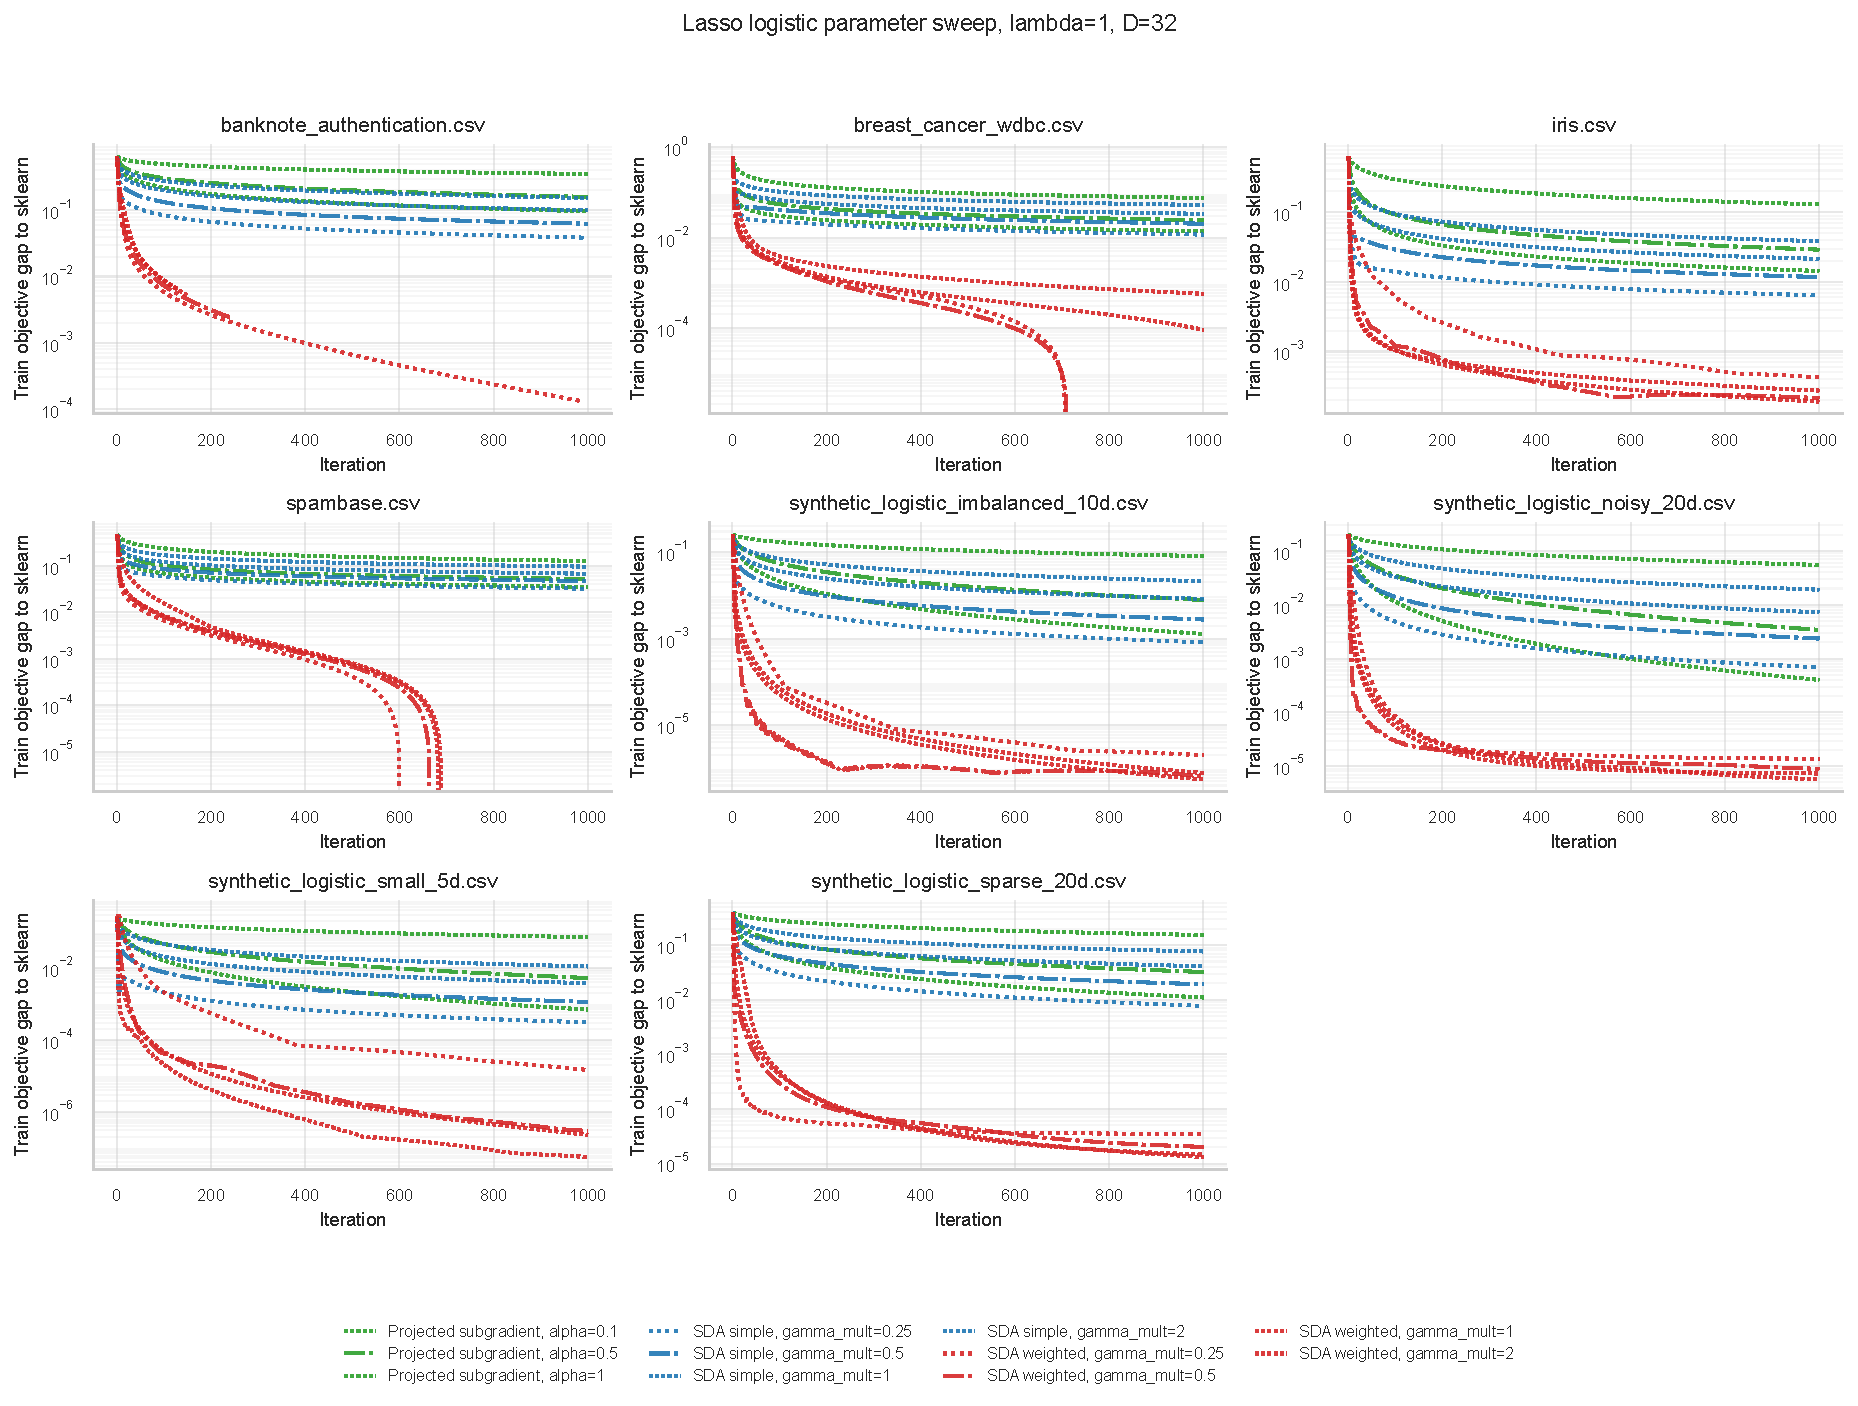
\includegraphics[width=\textwidth]{lasso_logistic_sparsity/lasso_parameter_sweep.pdf}
\caption{Step-parameter sweep for lasso logistic train-objective gaps at \(D=32\).}
\label{fig:lasso-param}
\end{figure}

\begin{figure}[htbp]
\centering
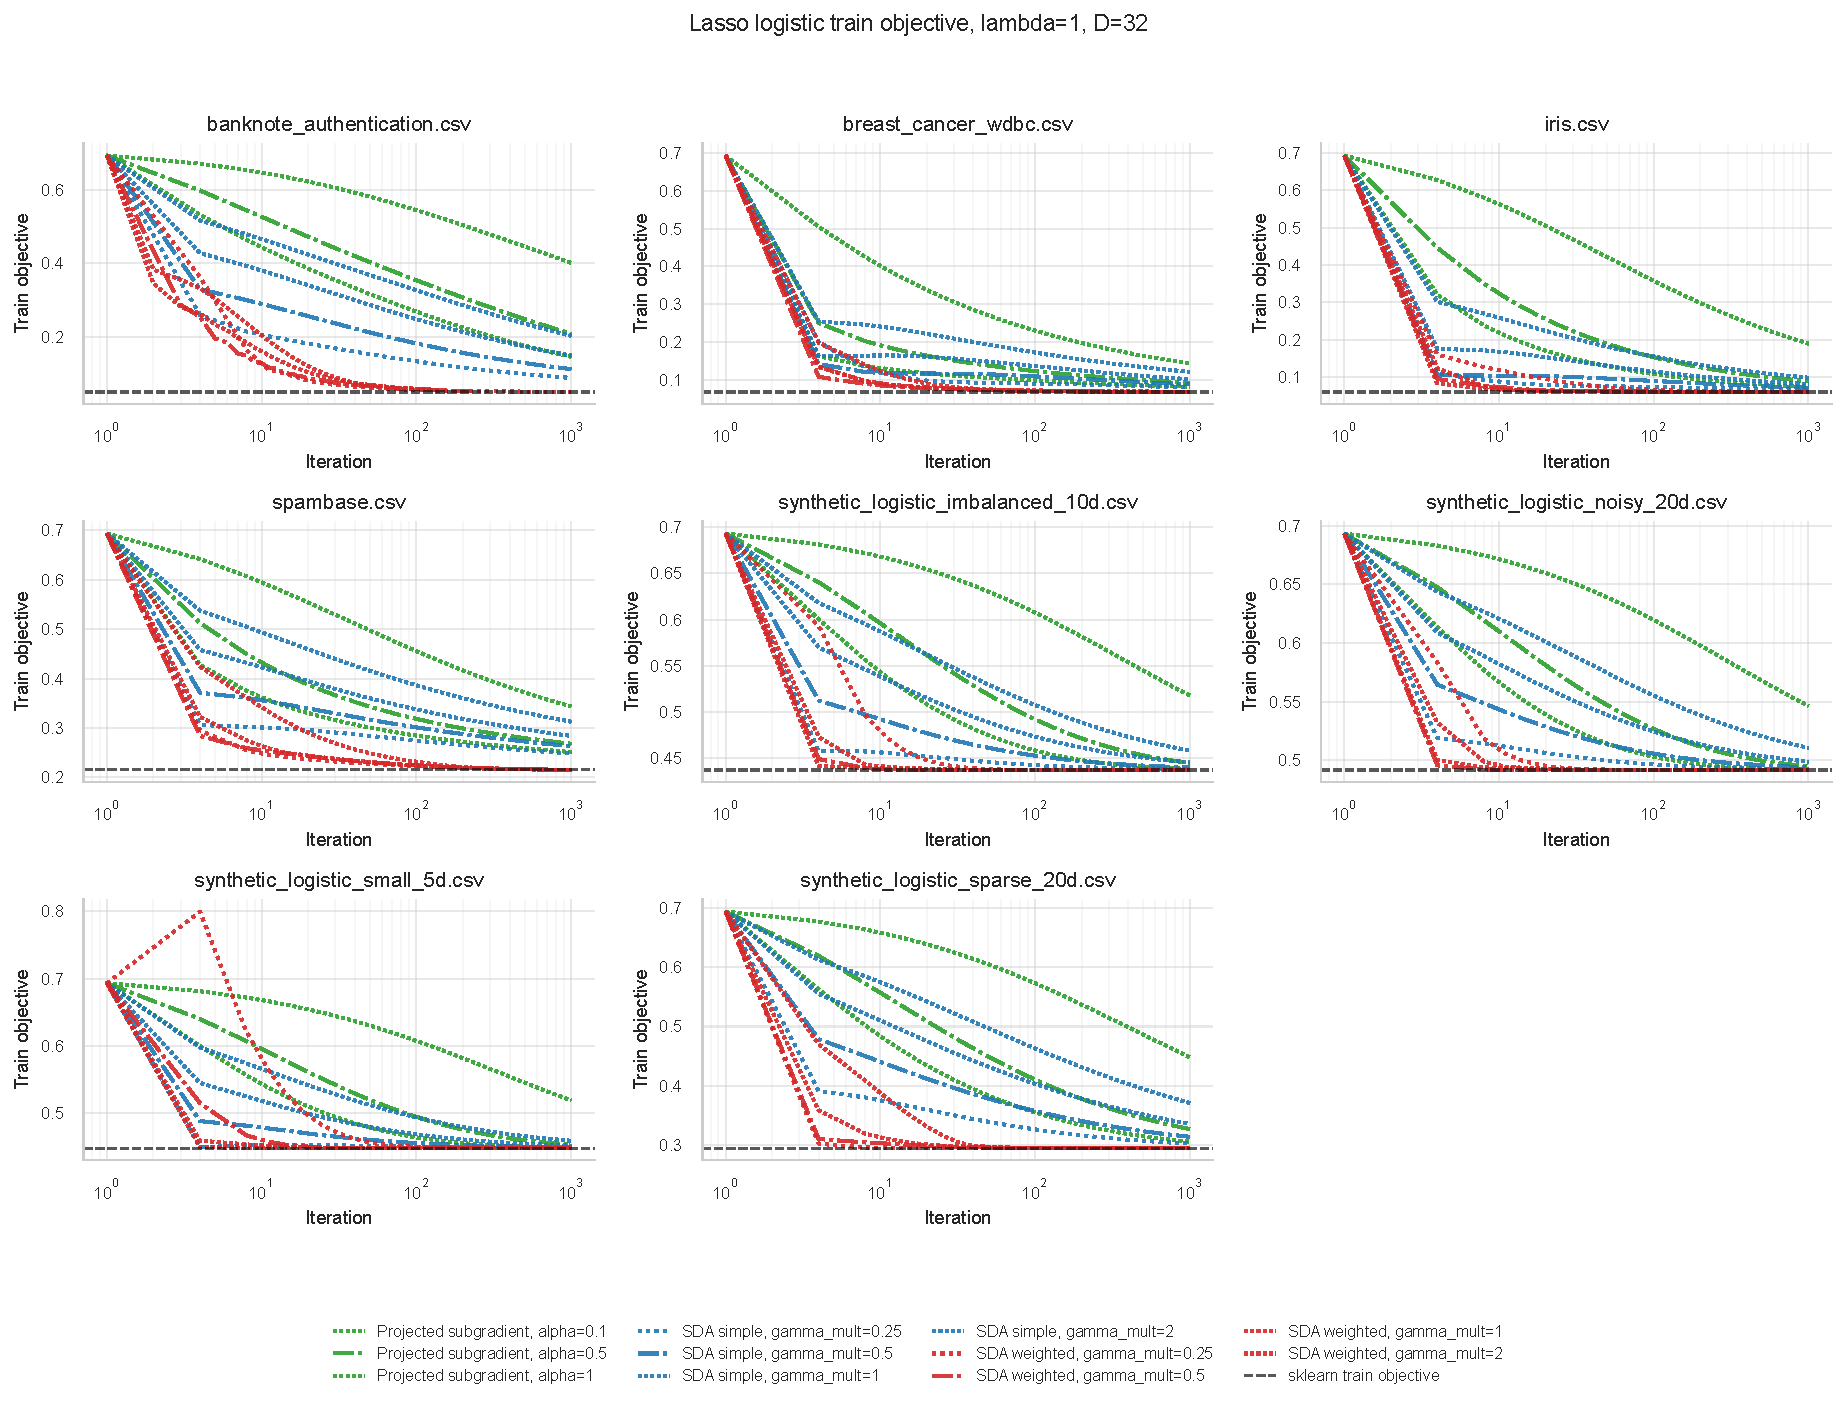
\includegraphics[width=\textwidth]{lasso_logistic_sparsity/lasso_parameter_sweep_train_objective.pdf}
\caption{Absolute train objectives for the lasso parameter sweep, with the sklearn SAGA reference.}
\label{fig:lasso-train}
\end{figure}

Figure~\ref{fig:lasso-norms} compares iterate norms against the SAGA solution
norm.  A decreasing train-objective gap does not require the iterate norm to match the
SAGA norm exactly, especially when the lasso problem has correlated features or
multiple nearly equivalent sparse predictors.  The norm plot is therefore used
as a diagnostic for scale and regularization behavior, not as a separate
optimality certificate.

\begin{figure}[htbp]
\centering
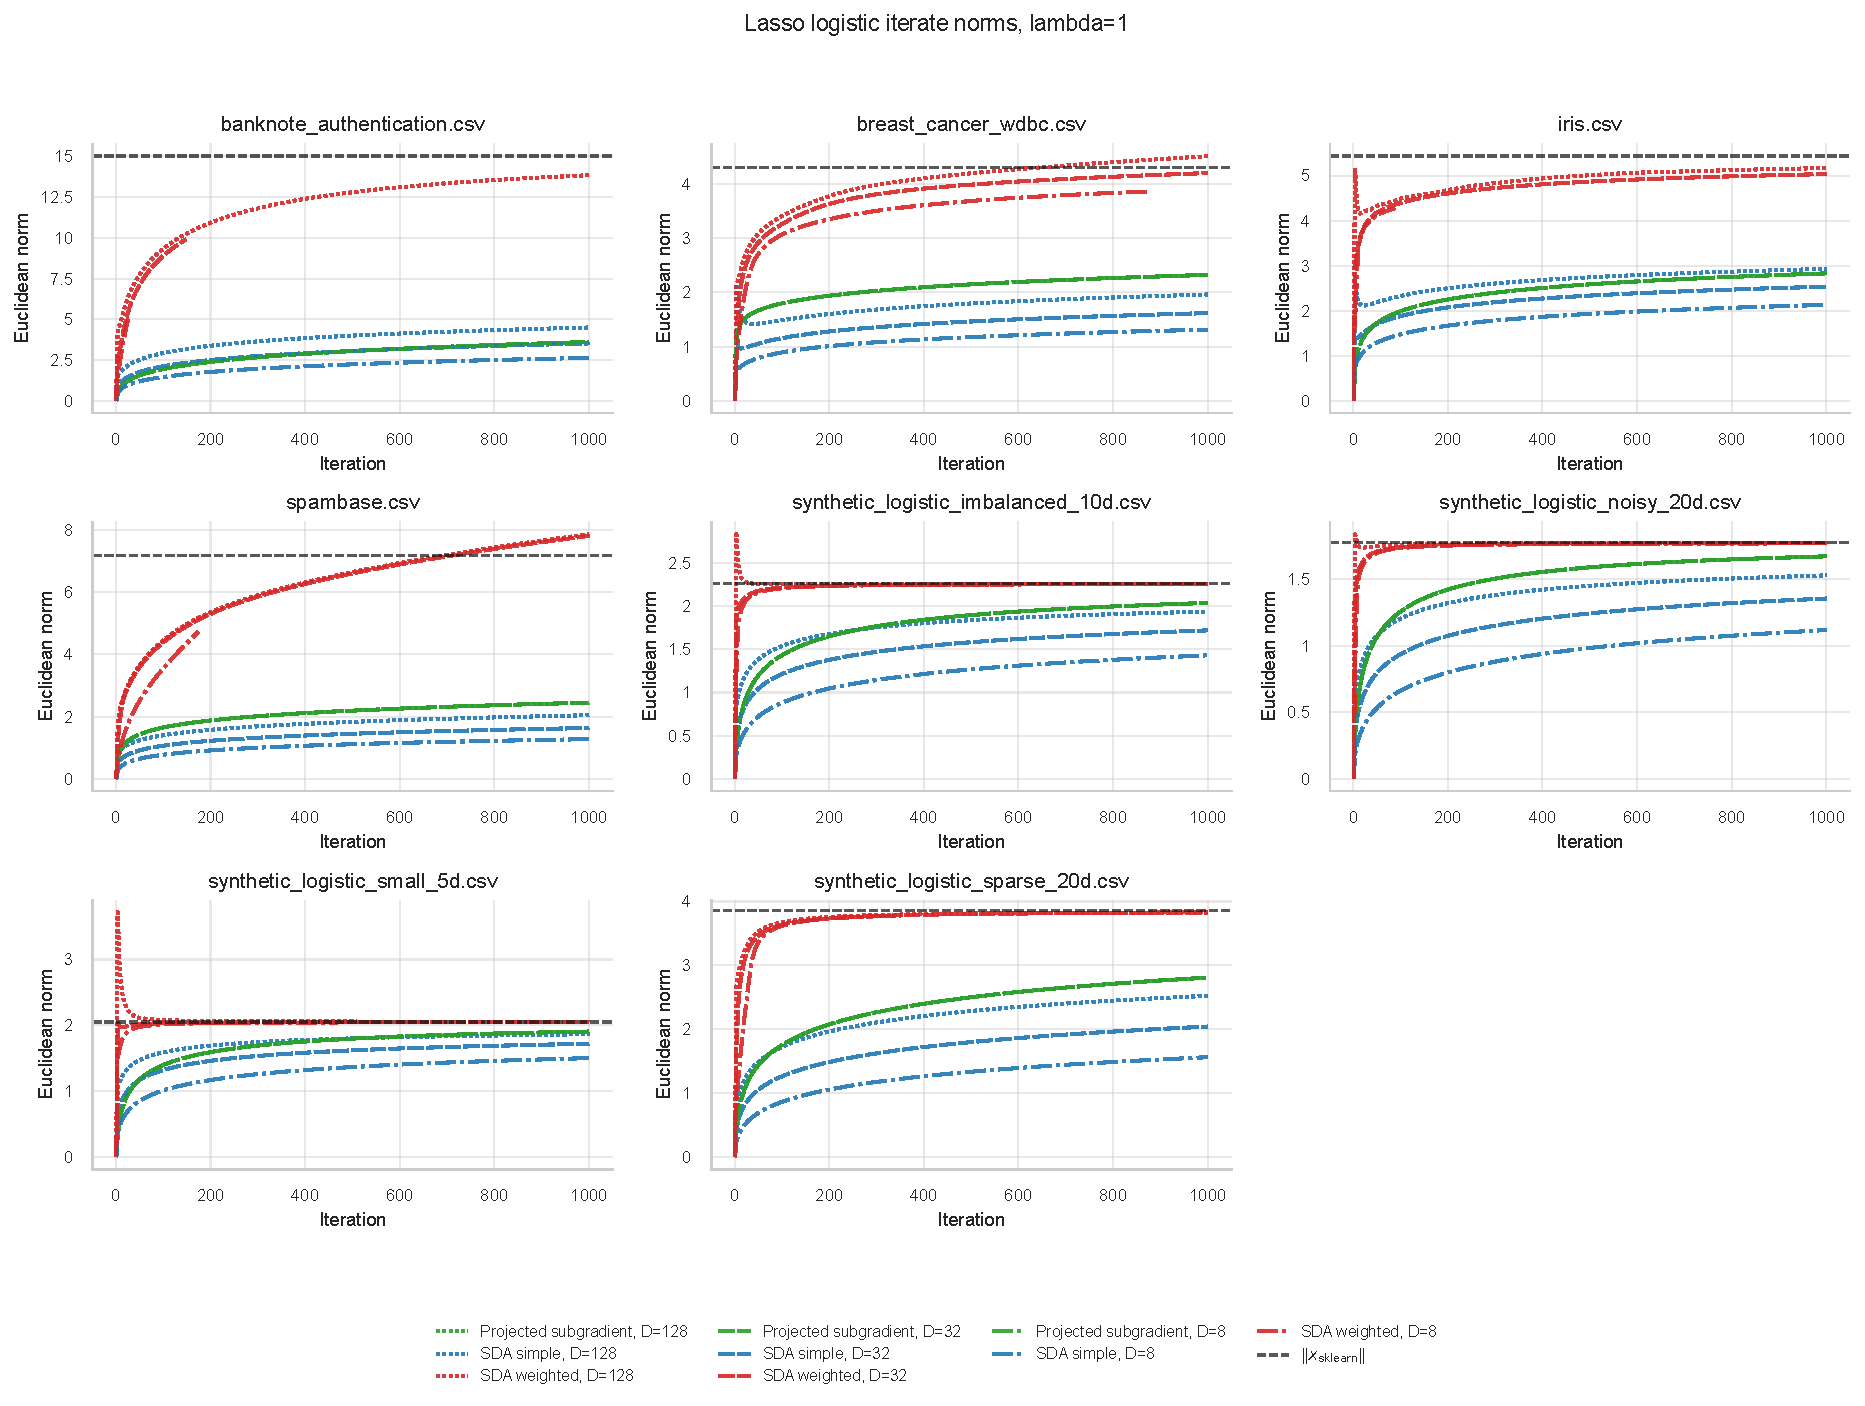
\includegraphics[width=\textwidth]{lasso_logistic_sparsity/lasso_norms.pdf}
\caption{Norms of lasso averaged iterates compared with the sklearn SAGA solution norm.}
\label{fig:lasso-norms}
\end{figure}

The runtime plot in Figure~\ref{fig:lasso-runtime} shows that sklearn SAGA is
faster on these small and medium lasso datasets, which is expected for a highly
optimized finite-sum solver.  Among the custom solvers, weighted SDA reaches
near-reference train objective values at runtimes comparable to the other custom
methods.  Since the SAGA reference is itself numerical, the runtime plot should
be interpreted as an empirical comparison to a strong implementation baseline,
not as a certificate of global optimality.

\begin{figure}[htbp]
\centering
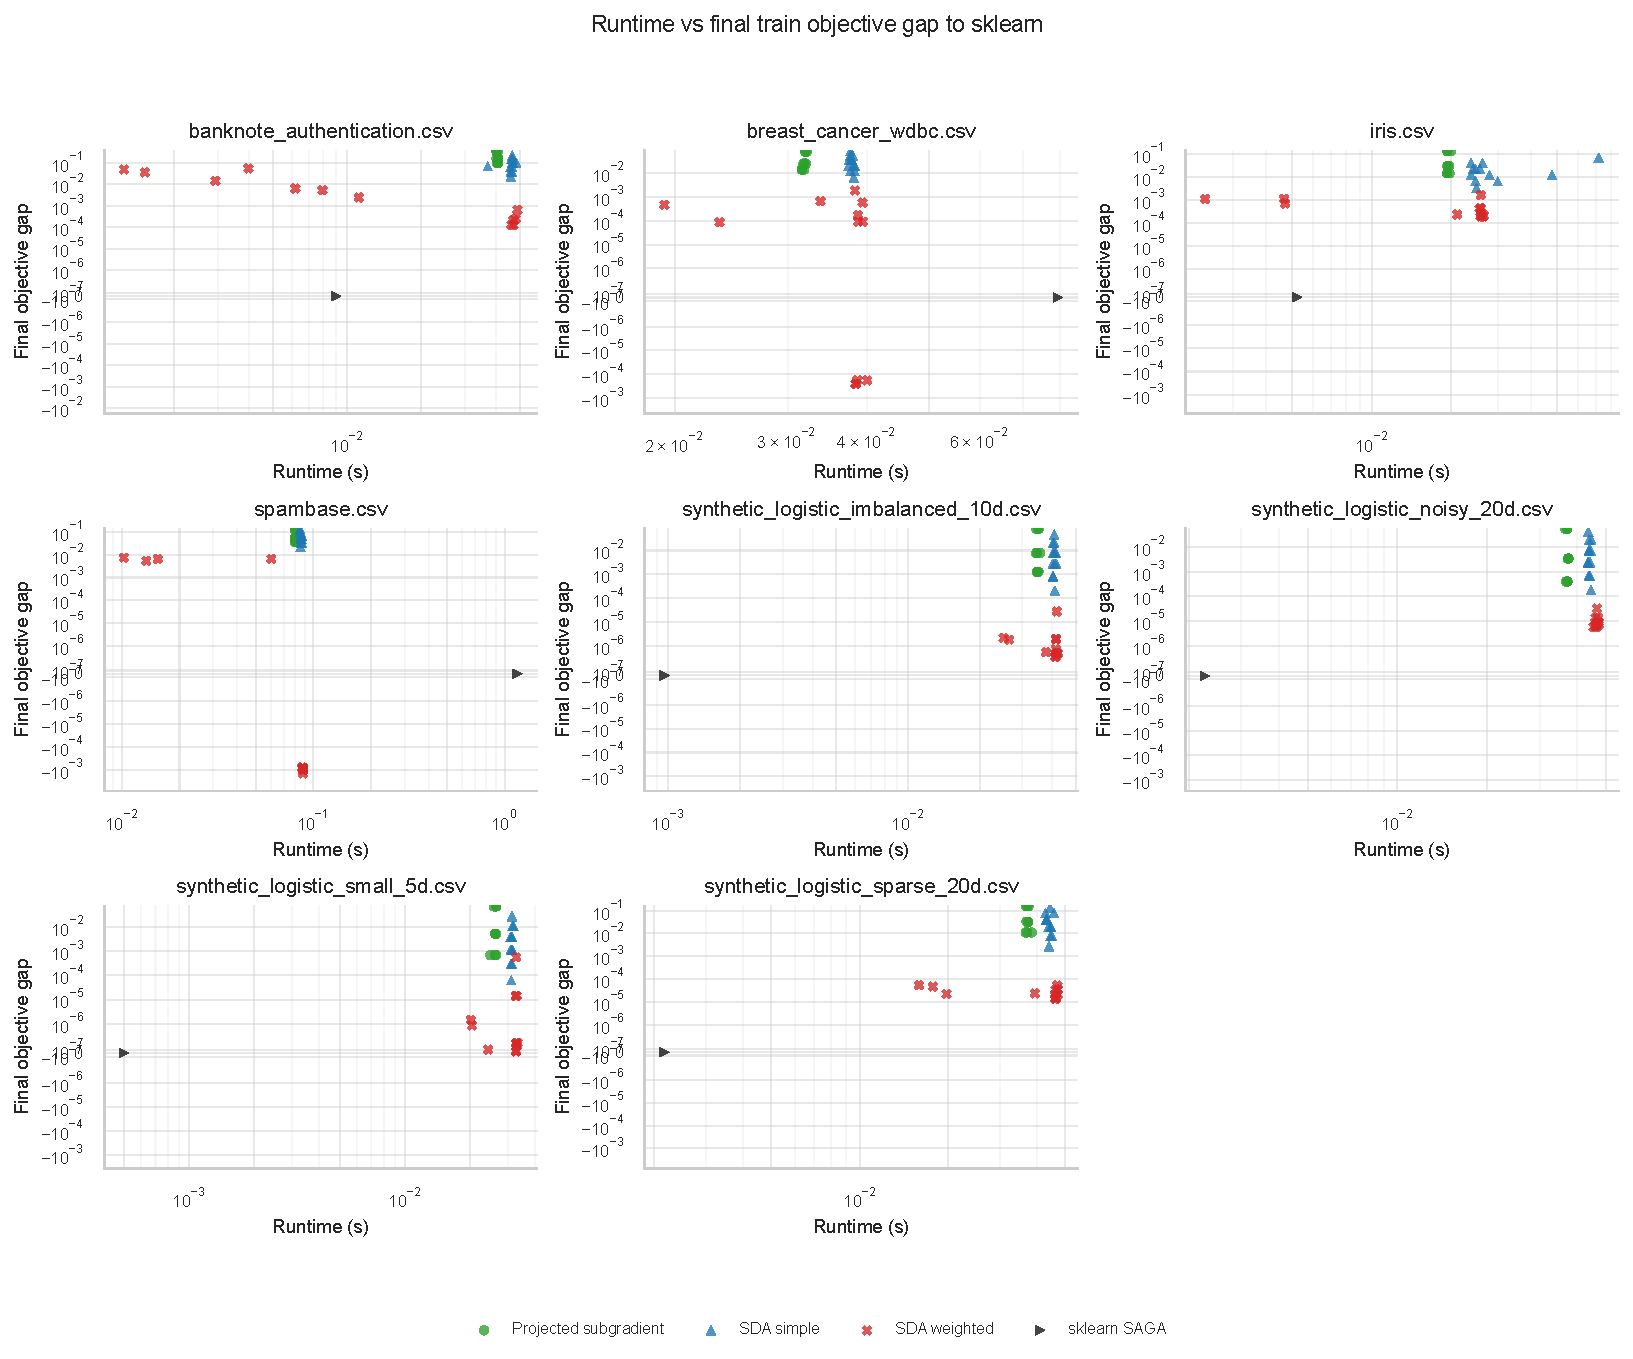
\includegraphics[width=\textwidth]{lasso_logistic_sparsity/lasso_runtime_vs_final_objective_gap_to_sklearn.pdf}
\caption{Runtime versus final train-objective gap to sklearn SAGA for lasso logistic datasets.}
\label{fig:lasso-runtime}
\end{figure}

\FloatBarrier

\subsection{Stochastic Simple Averages versus Weighted SDA on Synthetic Lasso}
\label{subsec:lasso-ssa}

\paragraph{Purpose and setup.}
The fifth experiment compares weighted full-gradient SDA with stochastic simple
averages (SSA) on synthetic lasso logistic datasets only.  The synthetic subset
contains the four original synthetic datasets and two larger generated
datasets: a sparse 50-dimensional problem with 12000 samples and a noisier
80-dimensional problem with 20000 samples.  The comparison fixes \(D=128\),
uses \(\lambda=1\), and sweeps \(\gamma_{\mathrm{mult}}\) values
\(0.25,0.5,1,2\).  SSA samples one training example per iteration and uses the
resulting stochastic subgradient in the simple dual-average update.  The
sampled subgradient is an unbiased estimator of the empirical logistic loss
gradient component, with the deterministic lasso subgradient added using the
same \(\lambda/n\) scaling as the full objective.

\begin{table}[htbp]
\centering
\small
\resizebox{\textwidth}{!}{%
\begin{tabular}{lrrrrr}
\toprule
Method & Runs & Median train-objective gap to SAGA & Best train-objective gap & Median runtime (s) & Median accuracy \\
\midrule
SDA weighted & 24 & \(6.95\cdot 10^{-6}\) & \(5.40\cdot 10^{-8}\) & \(4.57\cdot 10^{-2}\) & \(0.840\) \\
SSA & 24 & \(4.67\cdot 10^{-2}\) & \(1.53\cdot 10^{-3}\) & \(2.64\cdot 10^{-2}\) & \(0.828\) \\
sklearn SAGA & 6 & \(0\) & \(0\) & \(2.40\cdot 10^{-3}\) & \(0.840\) \\
\bottomrule
\end{tabular}
}
\caption{Synthetic-only SSA comparison.  Train-objective gaps are measured against matched sklearn SAGA.}
\label{tab:ssa-summary}
\end{table}

The runtime summary in Figure~\ref{fig:ssa-runtime} shows the main trade-off.
SSA is cheaper per iteration and has a lower median runtime than weighted SDA in
this grid, but its median final train-objective gap is much larger.  Weighted SDA is slower
because it evaluates the full training gradient, but on these synthetic
problems it reaches objective values much closer to the SAGA reference.  This is
mathematically consistent with stochastic approximation: a one-sample
subgradient has higher variance, so a fixed budget of 1000 iterations is not
expected to match a deterministic full-gradient method unless the cheaper
iterations are numerous enough or the step schedule is better tuned.

\begin{figure}[htbp]
\centering
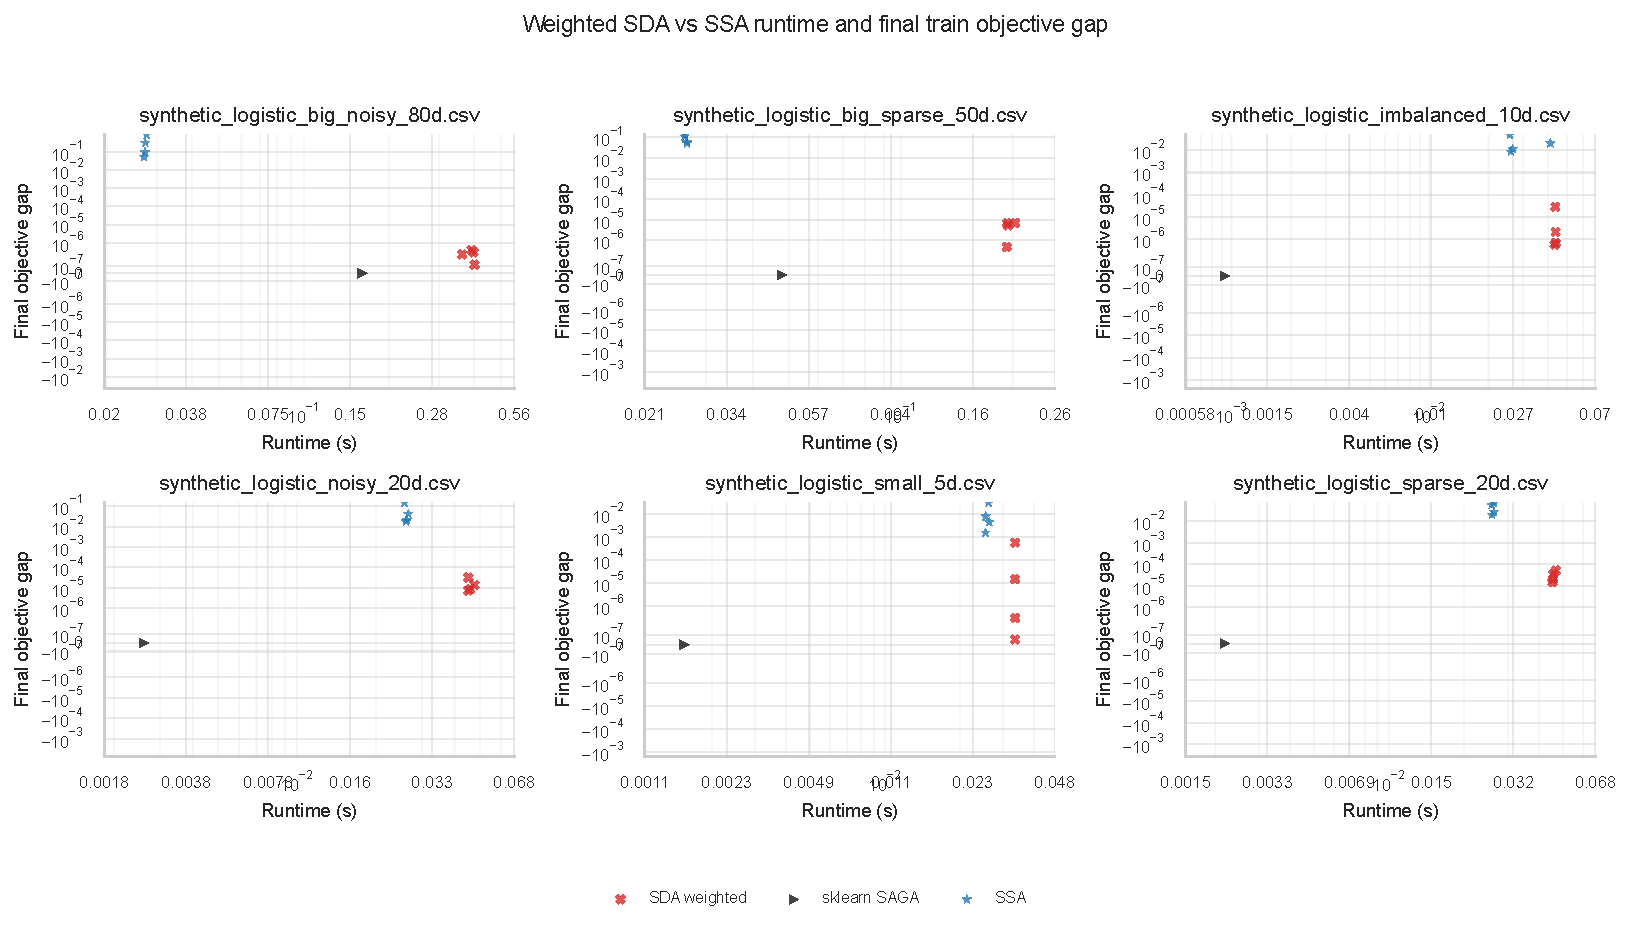
\includegraphics[width=\textwidth]{lasso_logistic_sparsity_ssa_comparison/lasso_ssa_runtime_vs_final_objective_gap_to_sklearn.pdf}
\caption{Runtime versus final train-objective gap for weighted SDA, SSA, and sklearn SAGA on synthetic lasso datasets.}
\label{fig:ssa-runtime}
\end{figure}

Figure~\ref{fig:ssa-param} shows the \(\gamma_{\mathrm{mult}}\) sweep.  The
weighted SDA curves usually descend rapidly toward the SAGA reference, while SSA
curves are noisier and flatten at larger train-objective gaps under the current iteration
budget.  The figure uses a logarithmic \(y\)-axis because the relevant
differences are multiplicative: train-objective gaps near \(10^{-6}\) and \(10^{-2}\) represent
qualitatively different optimization accuracy.

\begin{figure}[htbp]
\centering
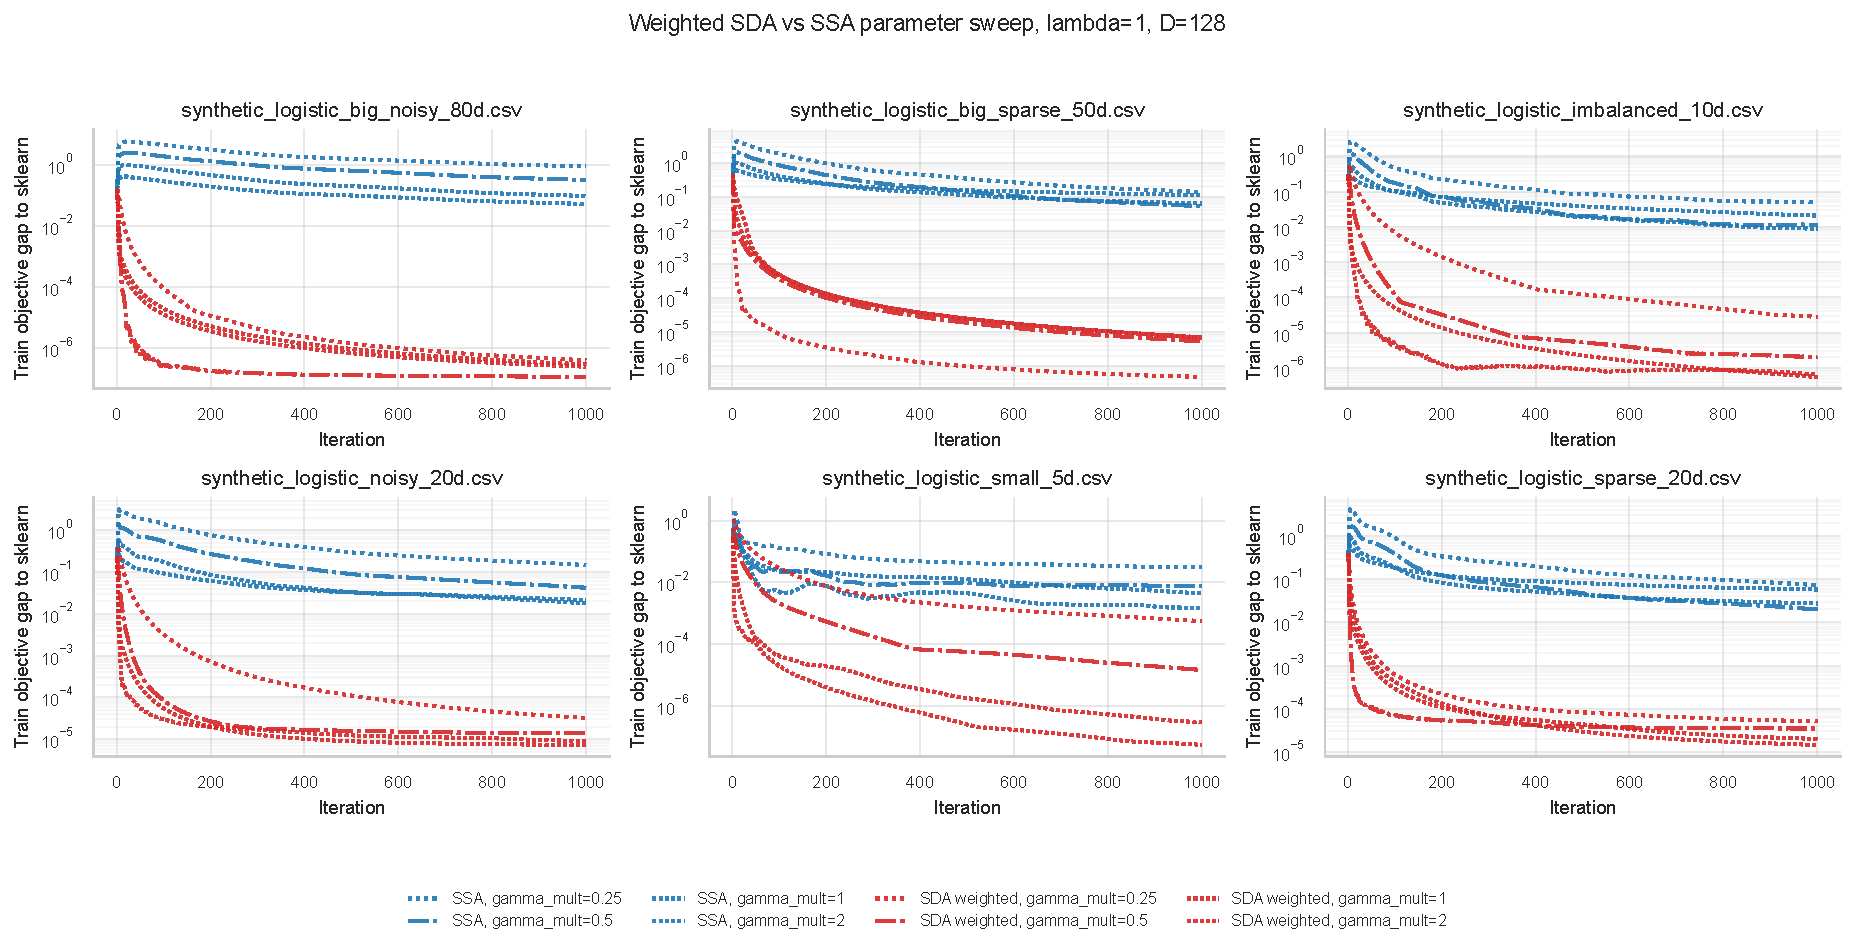
\includegraphics[width=\textwidth]{lasso_logistic_sparsity_ssa_comparison/lasso_ssa_parameter_sweep.pdf}
\caption{Step multiplier sweep for weighted SDA and SSA on synthetic lasso datasets.}
\label{fig:ssa-param}
\end{figure}

The absolute objective plot in Figure~\ref{fig:ssa-train} is a useful check on
the train-objective-gap plot.  The train objectives remain positive and are shown on a
logarithmic scale; the SAGA reference line indicates the empirical target.  On
the large synthetic datasets, the SSA trajectory still improves the objective
but does not close the train-objective gap to the same degree as weighted SDA.  Thus, for the
current implementation and budget, stochastic sampling reduces wall-clock cost
but does not compensate for the loss of full-gradient information.

\begin{figure}[htbp]
\centering
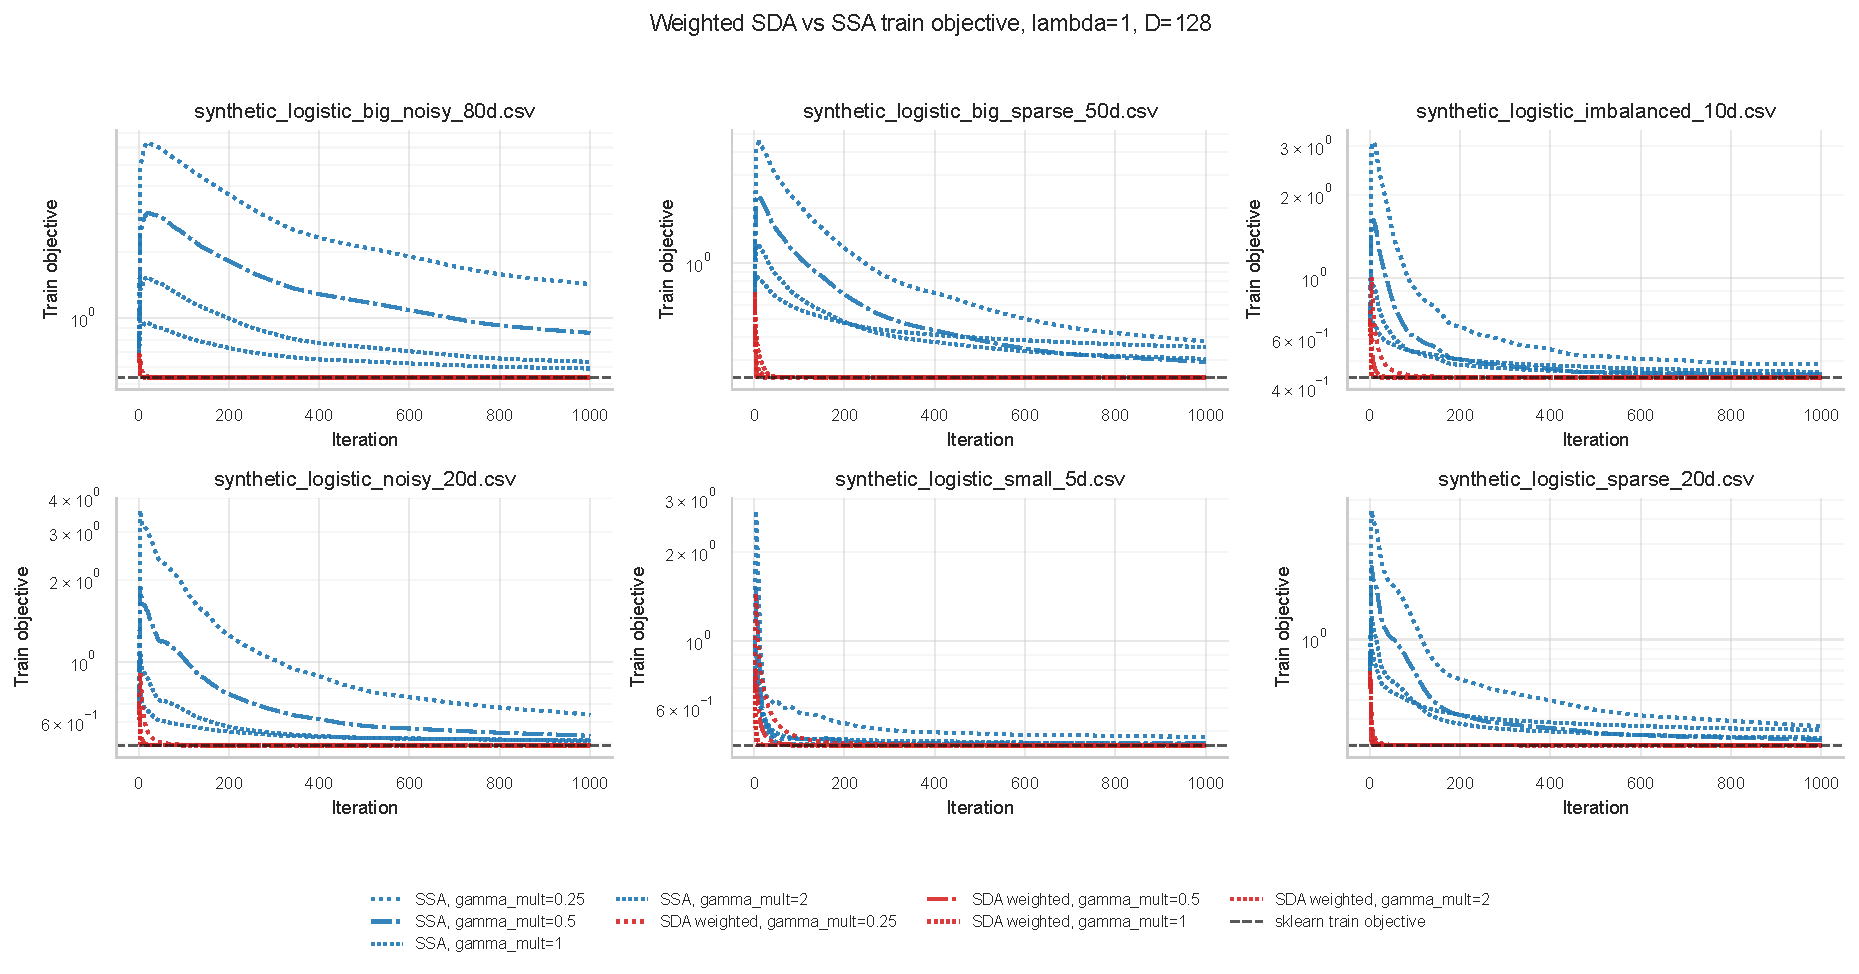
\includegraphics[width=\textwidth]{lasso_logistic_sparsity_ssa_comparison/lasso_ssa_parameter_sweep_train_objective.pdf}
\caption{Absolute train objective values for weighted SDA and SSA, with matched sklearn SAGA references.}
\label{fig:ssa-train}
\end{figure}

\FloatBarrier

\subsection{Cross-Experiment Discussion}
\label{subsec:cross-experiment}

Across the benchmark experiments, the plotted objective gaps are true objective
gaps to known optima.  Across the lasso experiments, the plotted gaps are
empirical train-objective gaps to sklearn SAGA.  These two types of objective
gap should not be conflated.  A true benchmark objective gap measures
mathematical suboptimality for the specified objective, whereas a lasso
train-objective gap measures agreement with a strong numerical reference.

Several conclusions are stable across the experiments.  First, the radius
prox-radius parameter \(D\) and step multiplier \(\gamma_{\mathrm{mult}}\) materially affect
SDA behavior; the experiments do not support a single universally best setting.
Second, weighted averaging is often helpful, especially in the lasso runs, but
it is not uniformly best on every nonsmooth benchmark or every prox geometry.
Third, geometry must match the problem: entropy prox is appropriate on the
simplex, while diagonal Euclidean prox helps only when its weights reflect the
objective anisotropy.  Finally, stochastic sampling should be evaluated by
runtime and final accuracy together.  In the present SSA comparison, cheaper
one-sample steps do not reach the same final objective accuracy as weighted
full-gradient SDA within the same 1000-iteration budget.

\begin{thebibliography}{9}

\bibitem{nesterov_primal_dual}
Y.~Nesterov.
\newblock Primal-dual subgradient methods for convex problems.
\newblock \emph{Mathematical Programming}, 120:221--259, 2009.

\bibitem{xiao_regularized_dual_averaging}
L.~Xiao.
\newblock Dual averaging methods for regularized stochastic learning and online optimization.
\newblock \emph{Journal of Machine Learning Research}, 11:2543--2596, 2010.

\bibitem{defazio_saga}
A.~Defazio, F.~Bach, and S.~Lacoste-Julien.
\newblock SAGA: A fast incremental gradient method with support for non-strongly convex composite objectives.
\newblock In \emph{Advances in Neural Information Processing Systems 27}, 2014.

\bibitem{koh_l1_logistic}
K.~Koh, S.-J. Kim, and S.~Boyd.
\newblock An interior-point method for large-scale \(\ell_1\)-regularized logistic regression.
\newblock \emph{Journal of Machine Learning Research}, 8:1519--1555, 2007.

\end{thebibliography}

\end{document}
